\documentclass[12pt,a4paper]{article}
\usepackage[utf8]{inputenc}
\usepackage[english]{babel}
\usepackage{amsmath}
\usepackage{amsfonts}
\usepackage{amssymb}
\usepackage{latexsym}
\usepackage{makeidx}
\usepackage{graphics}
\usepackage{lmodern}
\usepackage{hyperref}
\usepackage{subcaption}
\usepackage{pgfplots}
\usepackage{dsfont}
\usepackage{multicol}
\usepackage{xcolor}
\usepackage{booktabs}
\usepackage{float}
\usepackage{subcaption}
\pgfplotsset{width=10cm,compat=1.9}
\usepgfplotslibrary{external}
\usepackage{graphicx}
\usepackage{wrapfig}
\author{Daniel Vázquez Lago}
\usepackage{fancybox}
\title{Apuntes Electromagnetismo II}


\setlength{\parindent}{15px}
\usepackage[left=2.25cm,right=2cm,top=4cm,bottom=2cm]{geometry}


\newcommand{\parentesis}[1]{\left( #1  \right)}
\newcommand{\parciales}[2]{\frac{\partial #1}{\partial #2}}
\newcommand{\pparciales}[2]{\parentesis{\parciales{#1}{#2}}}
\newcommand{\ccorchetes}[1]{\left[ #1  \right]}
\newcommand{\D}{\mathrm{d}}
\newcommand{\derivadas}[2]{\frac{\D #1}{\D #2}}
\newcommand{\sech}{\mathrm{sech} \ }
\newcommand{\csch}{\mathrm{csch} \ }
\newcommand{\cotanh}{\mathrm{cotanh}}
\newcommand{\cotan}{\ \mathrm{cotan}}
\newcommand{\Res}{\mathrm{Res}}
\newcommand{\Arg}{\mathrm{arg}}
\newcommand{\Real}{\mathrm{Re}}
\newcommand{\tquad}{\quad \quad \quad}


\newcommand{\rota}{\nabla \times}
\newcommand{\dive}{\nabla \cdot}


\newtheorem{theorem}{Teorema}[section]
\newtheorem{corollary}{Corolario}[theorem]
\newtheorem{lemma}{Lema}[section]
\newtheorem{ejemplo}{Ejemplo}[section]

\begin{document}

\maketitle

\newpage

\tableofcontents

\newpage

\section{Analisis vectorial}

\section{Magnetostática}

\subsection{Fuerza de Lorentz}

¿Cuál es la principal cuestión que trata de contestar la electrodinámica? Como se mueven las cargas. Para esto es necesario conocer, dado un conjunto de cargas, que fuerza ejercen sobre otra carga. \\

Si las cargas están estáticas (...)

\begin{equation}
\vec{F} = q (\vec{E} + \vec{v} \times \vec{B})
\end{equation}

\subsection{Ley de Ampere}

La ley de Ampere nos permite calcular el campo magnético para problemas de muy alta simetría, usando el teorema de Stokes. El \textbf{teorema de Stokes} nos dice:

\begin{equation}
\oint_C \vec{F} \D \vec{l} = \int_S \rota \vec{F} \D \vec{S}
\end{equation}

siendo $\vec{F}$ un campo vectorial, y $S$ una superficie abierta de contorno $C$. Debemos tener en cuenta el \textit{sentido de circulación de C} para escoger la dirección de la normal de la superficie. Siempre escogeremos la normal tal que verifique la regla de la mano derecha. Entonces como:

\begin{equation}
\oint \vec{B} \D \vec{l} = \int_S \rota \vec{B} \D \vec{S} = \mu_0 \int_S \vec{J} \D \vec{S} = \mu_0 I_{enc}
\end{equation}

siendo $I_{enc}$ la intensidad que atraviesa la superficie S. Esta ley es extremadamente útil en problemas de simetría para los cuales podamos descartar ciertas direcciones y componentes de $\vec{B}$ y por lo tanto que a lo largo de la trayectoria cerrada $C$ $\vec{B}$ sea constante, y así podremos sacar $\vec{B}$ fuera de la integral. Ejemplos de esto es el cálculo de un hilo infinito, el campo de un toroide, de un cable coaxial, de un solenoide ideal...


\subsection{Ley de Biot-Savart}

Calculemos ahora el campo $\vec{B}$ directamente usando la expresión del potencial vectorial magnético tal que:

$$ \vec{B} = \rota \vec{A} = \rota \ccorchetes{\dfrac{\mu_0 I}{4 \pi} \oint \dfrac{\D \vec{l}'}{R}} $$

Sin embargo el rotacional implica la diferenciación respecto la posición del punto final, y dado que la integral es la integral de los puntos fuentes, podemos introducir el rotacional dentro de la integral:

$$ \vec{B} = \dfrac{\mu_0 I}{4 \pi} \oint  \rota \ccorchetes{\dfrac{\D \vec{l}'}{R}} $$


de donde se puede deducir que:

\begin{equation}
\vec{B} =  \dfrac{\mu_0 I}{4 \pi} \oint_C  \dfrac{\D \vec{l}' \times \vec{R}}{R^3} = \dfrac{\mu_0 }{4 \pi} \int_V  \dfrac{\vec{J}' \times \vec{R}}{R^3}  \D V'
\end{equation}




\newpage


\section{Magnetostática en medios materiales}
\newpage

\section{Electrodinámica clásica}

\subsection{Fuerza electromotriz}

\subsection{Ley de Faraday}

En 1820 se descubre que el magnetismo y la electricidad están intimamente relacionados, de tal forma que podemos decir que uno es completamente dependiente del otro. De este modo se desarrollo por Ampere toda la teoría que hemos visto ahora de magnetostática: una corriente eléctrica genera un campo magnético. Unos años después (1831), el físico inglés Michael Faraday se preguntó si el fenómeno inverso sucede, es decir, si un campo magnético genera una corriente eléctrica. Para responder a esta pregunta hizo unos experimentos, llegando a las siguientes conclusiones:

\begin{itemize}
\item Aparece una corriente eléctrica si movemos un circuito en presencia de un campo magnético constante a).

\item Aparece una corriente eléctrica si desplazamos el campo magnético constante (desplazamos el imán) dejando fijo el circuito b).

\item Aparece una corriente eléctrica si variamos la intensidad del campo magnético, dejando fijo el circuito c).
\end{itemize}

\begin{figure}[h!] \centering
\includegraphics[scale=0.7]{figura-griffiths-7.21.png}
\caption{Experimentos que realizó Faraday en 1831}
\end{figure}

Tras estos experimentos Faraday llegó, en un alarde de genialidad, a la siguiente conclusión: ``\textit{un campo magnético variable produce un campo eléctrico}'', de tal modo que denominó a este campo el \textit{campo eléctrico inducido} y a la diferencia de potencial que aparece en el circuito \textit{fuerza electromotriz inducida}, y se escribe como:

\begin{equation}
\varepsilon = - \dfrac{\D \phi}{\D t}
\end{equation}
donde $\phi$ es el flujo magnético.\\

En aquellos años no se había resuelto el problema de la fuerza que sufre una carga con velocidad $\vec{v}$ en presencia de un campo magnético, lo que hoy conocemos como ley de Loretnz. Sin embargo, si lo vemos en retrospectiva, podemos explicar los dos primeros experimentos usando esta ley. Por eso planteamos la siguiente pregunta: ¿Es suficiente la ley de Lorentz para explicar el experimento de Faraday?.

\subsubsection{¿Es suficiente la ley de Lorentz?}

Veamos el primer caso: tenemos un circuito magnético con velocidad $\vec{v}$ que se mueve respecto un campo magnético $\vec{B}$ constante en el tiempo. Si los portadores de carga se mueven con el circuito magnético, entonces por la ley de Lorentz aparece una fuerza por unidad de carga que llamaremos $\vec{f}_m$ tal que:

$$
\vec{f_m} = \vec{v} \times \vec{B}
$$

Si consideramos entonces que la velocidad y el campo magnético son perpendiculares entre si, además de ser perpendiculares al elemento de línea, podemos deducir que la fuerza electromotriz generada en nuestro circuito por esta fuerza será:

$$
\varepsilon = \oint f_m \D l = v B  l_0
$$
siendo $l_0$ el tramo de nuestro circuito que dicha relación de perpendicularidades se cumple. Es decir, podemos explicar que aparece una fuerza electromotriz con esta ley. \\

El segundo fenómeno también se puede explicar así si consideramos un cambio del sistema de referencia. Obviamente si consideramos que el circuito está quieto no podemos explicarlo así: no hay $\vec{v}$. Sin embargo, podemos hacer un cambio del sistema de referencia de tal manera que ahora nuestro problema es que se mueve el circuito, como el experimento uno. Esto último es muy interesante, ya que ya nos da una noción de lo que va a suceder después: las leyes del electromagnetismo son invariantes ante cambios de un sistema de coordenadas (incluso los relativistas!!). Esto que hemos estudiado es lo que comúnmente denominamos como \textbf{fuerza electromotriz debida al movimiento}, y se usa alrededor de todo el mundo para generar electricidad, trasformando la energía mecánica el electricidad. \\

Ahora bien, tratar de explicar el tercer experimento es bastante complicado. Ambos sistemas están quietos, por lo que surjen la siguiente preguntas: ¿Que sistema de referencia podemos usar ahora?¿Uno que se mueva con el campo magnético?¿Como se podría hacer esto?. La respuesta general es que no se puede, resulta muy complicado cambiar el sistema de referencia para que esto se cumpla. \\

Lo que si se verifica en este problema es la ley de inducción de Faraday. Si consideramos en este problema la variación del flujo como:

$$
\D \phi =  - \vec{B} \D \vec{A} = - B l_0 \D x = - B  l_0 v \D t 
$$

donde el signo menos viene de que el área del campo magnético disminuye, podemos ver fácilmente que:

\begin{equation}
\varepsilon = - \dfrac{\D \phi}{\D t}
\end{equation}

Entonces la ley de inducción de Faraday se verificará siempre, sin importar el sistema de coordenadas. Otro caso es que queramos considerar por separado la fuerza electromotriz debida al movimiento y la fuerza electromotriz generada por la variación de la intensidad del campo magnético, lo cual en cierto modo es lógico, ya que son fenómenos diferentes, pero teniendo una formulación del problema general, para que usar otra. 

\subsubsection{Universalidad de la ley de Faraday}

Supongamos los siguientes casos:

\begin{itemize}

\item \textbf{Caso estacionario:} en este caso el circuito estará en reposo, de tal modo que solo cambiará el campo magnético respecto al tiempo. Entonces tenemos que por la ley de faraday:

$$
\oint_C \vec{E} \cdot \D \vec{l} = \dfrac{\D }{\D t} \int_S \vec{B} \cdot \D \vec{A} = - \int_S \parciales{\vec{B}}{t} \cdot \D \vec{A} = \int_S (\nabla \times \vec{E}) \cdot \D \vec{A} 
$$ 
de tal manera que se verifica que:

\begin{equation}
\nabla \times \vec{E} = - \parciales{\vec{B}}{t}
\end{equation}


\item \textbf{Caso no estacionario:} el circuito está en movimiento, además de tener un campo magnético que cambia con el tiempo. Entonces existirán dos sistemas de referencia: aquel que se se mueva con el circuito ($\vec{E'}$) y aquel que no se mueve con el circuito ($\vec{E}$). Sabemos que en el segundo caso las cargas eléctricas sufrirán una fuerza tal que:

$$
\vec{F} = q (\vec{E}+\vec{v} \times \vec{B})
$$

Sin embargo en el otro sistema las cargas experimentarán una fuerza únicamente debidas a un campo eléctrico, de tal manera que:

$$
\vec{F}' = q \vec{E}'
$$

Las fuerzas tienen que ser iguales entre ellas (ya que tienen que tener la misma manifestación física), por lo que:

$$
\vec{E}' = \vec{E} + \vec{v} \times \vec{B}
$$

Sabemos que la potencia que el observador que está en reposo con el circuito medirá vendrá dada : 

$$
\varepsilon' = \oint_C \vec{E}' \cdot \D \vec{l} = - \int_S \parciales{\vec{B}}{t} \cdot \D \vec{A} + \oint_C (\vec{v} \times \vec{B}) \D \vec{l}
$$

Esto implica que:

$$
\int_S \nabla \times (\vec{E}' - \vec{v} \times \vec{B}) \D \vec{A} =  - \int_S \parciales{\vec{B}}{t} \D \vec{A}
$$

y si substituimos ahora este resultado por $\vec{E}$ obtenemos que:

\begin{equation}
\nabla \times \vec{E} = - \parciales{\vec{B}}{t}
\end{equation}

\end{itemize}


Es decir, hemos demostrado que la ley de inducción de Faraday y la ecuación de Maxwell completa se cumplen siempre, da igual el sistema de referencia que usemos. Incluso si la f.e.m. inducida viene dada por dos mecanismos completamente diferentes (como es la variación de la intensidad del campo magnético y la acción de la fuerza de Lorentz) tenemos que la estas dos ecuaciones son capaces de explicar la aparición de esta fuerza electromotriz. \\

\subsection{Ley de Lenz}

La ley de Lenz nos permite conocer de una manera cualitativa cual será el sentido de la corriente eléctrica en un circuito en la presencia de un campo magnético o flujo variable. La ley de lenz consta de un enunciado muy sencillo, tal que dice que: `` el sentido de la corriente es tal que se oponga al campo magnético que lo genera ''. Puede parecer un poco lioso, pero es bien sencillo. Según la regla de la mano derecha podemos intuir cual es la dirección del campo magnético generado por una espira. Pues entonces el sentido de la corriente de nuestro circuito será tal que el campo magnético que generaría esa corriente es opuesto al que entra. \\

De hecho es imposible que sea de otra forma, por el hecho de que en la ley de inducción de faraday aparece un signo negativo al lado del flujo. Supongamos que no existen densidades de cargas, por lo que $\nabla \vec{E} = 0$. Podemos suponer que $\vec{E}$ solo viene dado por su rotacional, y aplicando la fórmula integral de Ampere al campo eléctrico:

\begin{equation}
\oint_C \vec{E} \D \vec{l} = - \dfrac{\D \phi}{\D t}
\end{equation}
Si escogemos un flujo que sea positivo, por ejemplo eligiendo que el flujo positivo es el que atraviesa la espira en sentido $\widehat{z}$:

\begin{figure}[h!] \centering
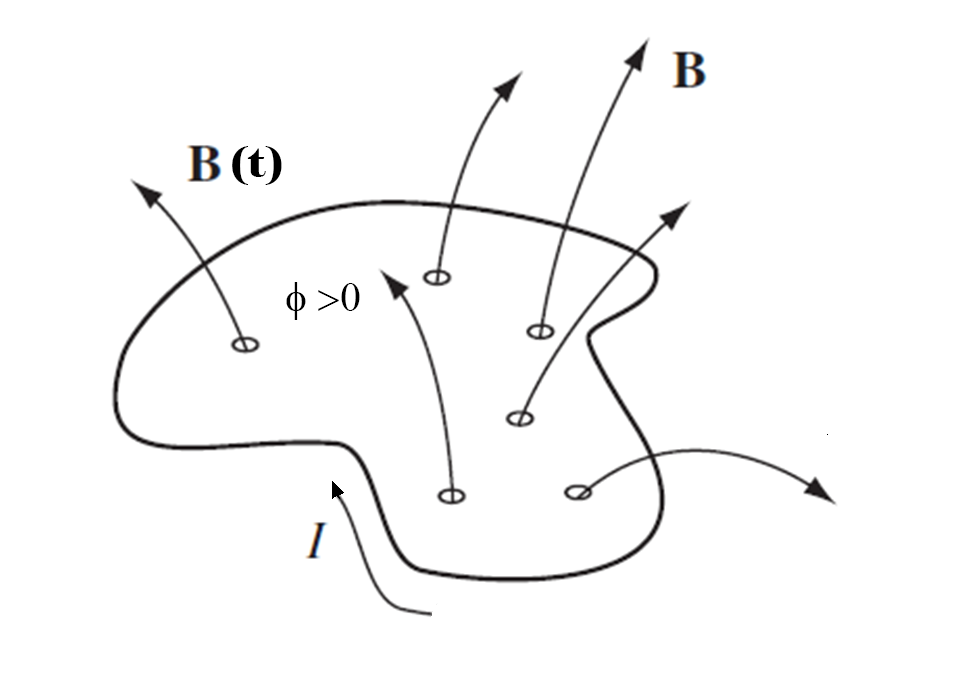
\includegraphics[scale=0.9]{espiras-lenz.png}
\end{figure}

y si cogemos la normal de la superficie también en el sentido del eje $z$ tenemos que el sentido de la circulación de $C$ en esa curva será horario, y como el lado derecho de la integral es negativo, tenemos que $\vec{E}$ y $\D \vec{ l}$ tienen que tener sentidos opuestos, es decir, la corriente se moverá en sentido anti-horario. Y según la mano derecha, la corriente que generaría sería en sentido $- \widehat{z}$, por lo que se verifica la ley de Lenz. 

\subsection{Coeficientes de inducción mutua} \label{Subsec:4.4}

Un circuito aislado recorrido por una corriente $i(t)$ es atravesado por su propio flujo magnético. Si este flujo varía con el tiempo se producirá una fuerza electromotriz determinada en el propio circuito, oponiéndose a la causa que lo produce. Aquí vemos claramente que tiene que tener un signo negativo la ley de Faraday (y por tanto la de Lenz), ya que de otra forma la fem generaría una corriente en el propio sentido de la corriente, aumentando $i(t)$ y generando energía del la nada, en un ciclo sin fin. Sin embargo este es un caso concreto de lo que llamamos \textit{inductores} e \textit{inductancias}. Entones:

\begin{equation}
\varepsilon_{ind} = - \dfrac{\D \phi}{\D t} = - \dfrac{ \D \phi}{\D i} \dfrac{\D i}{t}
\end{equation}

Al término $\dfrac{\D \phi}{\D i}$ se le llama el \textbf{coeficiente de autoinductancia} del circuito. Si este es constante podemos relacionar el flujo directamente con la intensidad además de

\begin{equation}
\varepsilon_{ind} = - L \dfrac{\D i}{\D t}
\end{equation}

Las unidades del coeficiente de autoinducción son los Henrios. Este concepto se puede extender a sistemas en los que haya varias espiras en el espacio, como vamos a ver a continuación. \\

Consideremos dos espiras cerradas y cercanas $c_1$ y $c_2$ que encierran unas superficies abiertas $S_1$ y $S_2$. Supongamos que cada espira tiene intensidad $i_1$ e $i_2$, creando unos campos $\vec{B_1}$ y $\vec{B_2}$. Algunas lineas de $\vec{B_1}$ pasarán por la superficie $S_2$. Entonces existirá un flujo magnético que pase por dicha superficie, que si varía con el tiempo generará una fuerza electromotriz inducida en la espira. El flujo que atraviesa dicha superficie se puede calcular como:

\begin{equation}
\phi_{12} = \int_{S_2} \vec{B_1} \D \vec{S_2}
\end{equation}
y si tenemos en cuenta que $\int \vec{B_1} \D \vec{S_2} = \oint \vec{A_1} \D \vec{l_2}$ y escribimos $\vec{A_1}$ según la expresión del potencial vectorial de Helmholtz tenemos que:

\begin{equation}
\phi_{12} = \oint_2 \vec{A_1} \D \vec{l_2} = \oint_2 \parentesis{\dfrac{\mu_0 I_1}{4 \pi} \oint \dfrac{\D \vec{l_1}}{R}} \cdot \D \vec{l_2} = \dfrac{\mu_0 I_1}{4 \pi} \oint_2 \oint_1 \dfrac{\D \vec{l_1} \D \vec{l_2}}{R}
\end{equation}
donde definimos como \textbf{coeficiente de inducción mutua} entre dos circuitos a

\begin{equation}
M_{12} = \dfrac{\mu_0}{4 \pi} \oint_1 \oint_2 \dfrac{\D \vec{l_1} \cdot \D \vec{l_2}}{R}
\end{equation}

Y ahora podemos escribir la ecuación del flujo como:

\begin{equation}
\phi_{12} = M_{12} I_2
\end{equation}

Como se puede ver el coeficiente de inducción mutua (cuya expresión es conocida como la \textit{ecuación de Newmann}) es simétrico respecto a los subíndices 1 y 2 (podemos intercambiar las integrales y el producto escalar), por lo que:

\begin{equation}
M_{12} = M_{21}
\end{equation}

En este caso el término siguiente es equivalente a la autoinductancia:

\begin{equation}
L_1 = M_{11} = \dfrac{\mu_0}{4 \pi} \oint_1 \oint_1 \dfrac{\D \vec{l_1} \cdot \D \vec{l_1} }{r}
\end{equation}

Este coeficiente no es una forma muy útil para el cálculo, pero que revela algunas propiedades del coeficiente de inducción mutua, que son:

\begin{itemize}

\item Son factores puramente geométricos.

\item $L >0 $, por la ecuación de Lenz. Si fuera negativo se podría crear energía de la nada. Además podemos considerar que $L$ ejerce un papel similar a la masa en la mecánica: a mayor coeficiente $L$ mas difícil resulta hacer cambiar la intensidad de un circuito. 

\item Los coeficientes $M_{ij}$ pueden ser positivos o negativos, en función de como se recorran los circuitos. Siempre se cumple que $|M_{ij}| \leq L$. 

\item Para un sistema de $N$ circuitos tenemos que el flujo que atraviesa un circuito $i$ concreto vendrá dado por: $ \phi_i = \sum_{j=1}^N M_{ij} i_j $

\end{itemize}


\subsection{Aplicaciones}

Las aplicaciones de la ley de Faraday son tremendas, sin embargo las dos mas importantes son las que vamos a ver a continuación: el trasformador y el generador de corriente alterna.

\subsubsection{Trasformador}

Un trasformador es un dispositivo de corriente alterna que nos permite trasformar voltajes, corrientes e impedancias. Normalmente consiste en dos o más bobinas acopladas magnéticamente a través de un núcleo ferromagnético común.\\



\begin{wrapfigure}{l}{0.35\textwidth}
    \centering
    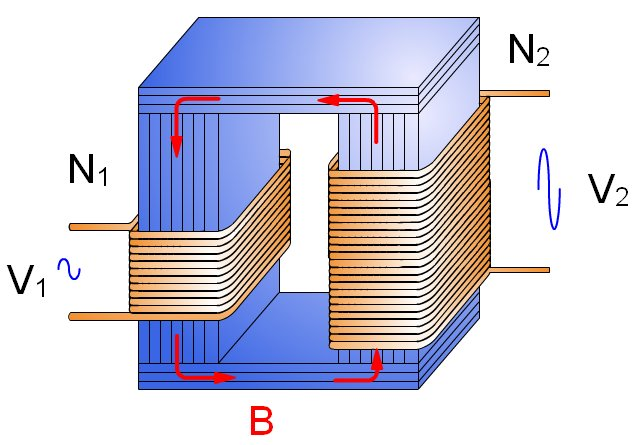
\includegraphics[width=0.35\textwidth]{trasformador.jpg}
    \caption{Trasformador}
\end{wrapfigure}


Entonces sobre este núcleo ferromagnéticos enrollamos dos bobinas, una llamada la bobina primaria y otra la secundaría. El funcionamiento será el siguiente: por la bobina primaria va a pasar una intensidad que cree un campo magnético. Debido a que está enrollado sobre un núcleo ferromagnético todo el campo magnético $\vec{B}$ estará encerrado por dicho material.vAl pasar el campo magnético a travesará el bobinado secundario. Si dicho flujo magnético dependiera del tiempo, se generaría una corriente magnética en el bobinado secundario con una potencia menor (si $N_1 < N_2$) o mayor (si $N_1 > N_2$).  \\

Podemos aplicar la teoría de circuitos magnéticos a este problema.

\begin{equation}
N_1 I_1 - N_2 I_2 = \mathfrak{R} \cdot \phi
\end{equation}

(negativo porque las intensidades tendrán diferentes sentidos). Si el trasformador es perfecto y no se producen pérdidas de ningún tipo (no se escapan las lineas de campo) tenemos que $\mu \rightarrow \infty$ y $\mathfrak{R} \rightarrow 0$, por lo que se verificará:

\begin{equation}
N_1 I_1 = N_2 I_2
\end{equation}
de lo que se puede deducir que

\begin{equation}
\dfrac{I_2}{I_1} = \dfrac{N_1}{N_2} \label{Ec:4-trasformador}
\end{equation}
y como consecuencia de la ley de Farday que nos dice que la fuerza electromotriz de los bobinados son:

\begin{equation}
V_1 = N_1 \dfrac{\D \phi}{\D t}; \tquad V_2 = N_2 \dfrac{\D \phi}{\D t}
\end{equation}
tenemos que podemos reescribir la ecuación \ref{Ec:4-trasformador} como:


\begin{equation}
\dfrac{I_2}{I_1} = \dfrac{N_1}{N_2} = \dfrac{V_1}{V_2}
\end{equation}

Sin embargo en los trasformadores reales esto no sucede así. Existe flujo de fuga, inductancias finitas y resistencia distinta de cero en el circuito, la presencia de histéresis y pérdidas por corrientes parásitas. Además la naturaleza no lineal del núcleo ferromagnético (depende de la intensidad del campo magnético) hace complicado este problema. \\

El fenómeno de las corrientes parásitas es un fenómeno no buscado en los trasformadores. Este se produce por la propia ley de inducción de Faraday. La existencia de un campo magnético variable producirá corrientes locales en el propio núcleo del conductor, lo que producirá una pérdida ohmica de potencia y calor. Una manera de evitar esto es buscar materiales con alta permeabilidad y baja conductividad. A estos materiales los llamamos \textit{ferritas}. Otra manera de evitar las corrientes parásitas es crear el trasformador a partir de láminas de hierro apiladas separadas por un barniz aislante, de tal manera que el recubrimiento sea paralelo a la dirección del flujo magnético (primera disposición de la figura). Si el recubrimiento es perpendicular (segunda disposición) el efecto pasará desapercibido. La pérdida total se reducirá aumentando el número de laminas. En general depende de la forma y tamaño de la sección trasversal, así como del tipo de laminado. \\

Aunque la pérdida por corrientes parásitas no sea un fenómeno buscado en los trasformadores, este funcionamiento es lo que permite que existan cocinas de inducción y en general calentamiento por inducción. \\

\begin{figure}[h!]
    \centering
    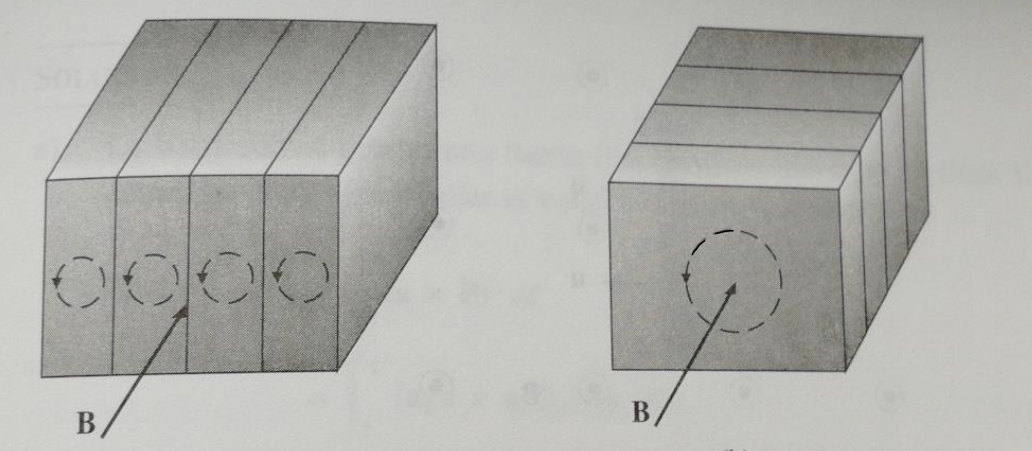
\includegraphics[scale=0.5]{laminacion.png}
    \caption{ciclo histéresis}
\end{figure}




\newpage

\section{Energía y fuerzas}

\subsection{Energía en campos magnéticos}

Como sabemos cuesta una energía poner a funcionar una corriente en un circuito. En un circuito hay en juego dos energías: la que se consume en forma de calor por las resistencias y otra que representa el trabajo que se realiza por las baterías en contra de la f.e.m. inducida, y que es la que permite que exista una corriente. El trabajo que se realiza en contra de la fuerza electromotriz inducida para mantener dicha corriente será:

\begin{equation}
\dfrac{\D W}{\D t} = - \varepsilon I = L \cdot I \cdot \dfrac{\D I}{\D t}
\end{equation}
que se puede reescribir como:

\begin{equation}
\dfrac{\D W}{\D t} =  \dfrac{\D \phi}{\D t} I \Longrightarrow \D W = I \D \phi
\end{equation}

El trabajo que se pone en juego para crear una corriente $I$ en un tiempo $t$ será de:

\begin{equation}
W = \dfrac{1}{2} L I^2 = \dfrac{1}{2} I \phi
\end{equation}
por lo que el trabajo dependerá únicamente de la geometría y de la corriente final del circuito. Esto se puede reescribir como:

$$ W = \dfrac{1}{2} I \int_S \vec{B} \D \vec{S} = \dfrac{1}{2} I \oint_C \vec{A} \D \vec{S}
=  \dfrac{1}{2} \oint_C \vec{A} I \D \vec{S} $$ 


Generalizando para una corriente volumínica:

\begin{equation}
W = \dfrac{1}{2} \int_V (\vec{A} \cdot \vec{J}) \D \tau \label{Ec:5.1-022}
\end{equation}
que si usamos que $\nabla \times \vec{B} = \mu_0 \vec{J}$ y la regla de la cadena podemos obtener que

$$ W = \dfrac{1}{2 \mu_0} \int_V (\vec{A} \cdot \vec{J})  \D \tau = \dfrac{1}{2 \mu_0} \int_V B^2 \D \tau + \dfrac{1}{2 \mu_0} \oint_S(\vec{A} \cdot \vec{B})   \D S $$

Dado que el segundo término tenderá a cero (sabemos que $A \propto 1/r, B \propto 1/r^2$) cuando la región integrada tienda a ocupar todo el universo, tenemos finalmente la expresión de la energía. 

\begin{equation}
W = \dfrac{1}{2 \mu_0} \int_{univ} B^2 \D \tau \label{Ec:5.1-023}
\end{equation}
por lo tanto tenemos que la energía está almacenada o bien en los campos \ref{Ec:5.1-022} o bien en las corrientes que los producen \ref{Ec:5.1-023}, pero ambas son equivalentes entre sí. \\

Como ya sabemos un campo $\vec{B}$ no produce trabajo, al no alterar la energía cinética de las cargas en su presencia. Sin embargo acabamos de comprobar que para crear un campo magnético cuesta energía. La explicación es la ley de Faraday: para producir un campo $\vec{B}$ hace falta cambiarlo, y cambiar un campo magnético induce directamente un campo $\vec{E}$ que sí cuesta energía. Hay cierto paralelismo con la energía almacenada por el campo eléctrico:

\begin{equation}
\begin{array}{lllllll}

W_{elec} & =  & \frac{1}{2} \int V \cdot \rho \D \tau & = & \frac{\varepsilon_0}{2} \int E^2 \D \tau & = & \dfrac{1}{2} \ \int_V \vec{E} \vec{D} \D \tau \\ \\

W_{mag} & = & \frac{1}{2} \int \vec{A} \cdot \vec{J} \D \tau & = & \frac{1}{2\mu_0} \int B^2 \D \tau & = & \dfrac{1}{2} \ \int_V \vec{B} \vec{H} \D \tau

\end{array}
\end{equation}

\subsubsection{Energía de un sistema de corrientes}

Crear un sistema de corrientes cuesta un trabajo, que podemos ver como la cantidad de trabajo que cuesta hacer aparecer determinada corriente en el infinito y llevarla al punto donde se encuentra en el sistema final. Podemos aplicar las ecuaciones anteriores para calcular esta energía, ya que podemos convertir la ecuación \ref{Ec:5-Energiacorrientes} en una suma de corrientes discretas $\int_V \vec{J} \D \tau = i \int \D \vec{l}$ . Además si tenemos en cuenta que $$ \int \vec{A} \D \vec{l} =\int_S (\nabla \times \vec{A})\D \vec{S} = \int \vec{B} \D \vec{S}  = \phi_M$$tenemos que: 

\begin{equation}
W_m = \dfrac{1}{2} \sum_{k=1}^N \sum_k i_k \phi_k
\end{equation}
por otra parte sabemos que el flujo que atraviesa un circuito cualquiera viene determinado por los coeficientes de inductancia y la intensidad de los demás circuitos. Esto nos lleva a escribir la energía almacenada en un sistema de corrientes como:

\begin{equation}
W_m = \dfrac{1}{2} \sum_{k=1}^N  \sum_{j=1}^N i_k i_j M_{kj}
\end{equation}

\subsection{Fuerzas magnéticas sobre circuitos}

Como sabemos dos corrientes en general ejercerán fuerzas entre sí, que se pueden calcular usando leyes ya vistas. Sin embargo en algunos ejercicios y problemas resulta conveniente expresar la fuerza en términos de variaciones de energía. Para que un sistema de corrientes este fijo en el espacio, sin moverse, va a tener que aparecer una fuerza mecánica $F_{mec}$ externa igual que la fuerza magnética $F_m$ que se ejerzan entre sí los circuitos. Esta fuerza tiene que ser igual en módulo y con dirección opuesta a $F_m$: \\

\begin{equation}
\vec{F}_m = -  \vec{F}_{ext}
\end{equation}

A partir de ahora vamos a usar un principio, el principio de los trabajos virtuales. Sabemos que la variación de energía cinética en un sistema es igual al trabajo realizado por todas las fuerzas 

\begin{equation}
\Delta T = W_{ext} + W_{b} + W_{mag}
\end{equation}

Pero al considerar un trabajo virtual tenemos que el proceso será completamente cuasiestático, es decir, en completo equilibrio, de tal modo que se pueda desplazar una cantidad $\delta r$ tan infinitamente despacio que $\delta T = 0$. Viendo lo que significa cada término:

\begin{itemize}
\item $W_{ext}$: es la energía que aporta la fuerza externa. Como es conservativa viene dada por: 

$$W_{ext} = - \Delta U_{ext} = \int \vec{F}_{ext} \vec{\D r} $$

\item $W_{b}$: es la energía que aportan las baterías para mantener la corriente eléctrica. Viene dada por la siguiente ecuación ya que es la energía que hace falta suministrar para mantener la intensidad constante en contra de la fem inducida.

$$W_{b} = \sum_i I_i  \cdot \phi_i  \Longrightarrow \D W_b = \sum_i I_i \cdot \D \phi_i $$ 

\item $W_{m}$: es la energía que aportan las fuerzas magnéticas entre los circuitos. Como es conservativa viene dada por: 

$$W_{m} = - \Delta U_{m} = \int \vec{F}_{m} \vec{\D r} $$


\end{itemize}


Antes de ver como se comporta la fuerza es importante mencionar que lo que denotamos como $U$ no es mas que un potencial, la energía potencial. Ahora vamos a estudiar que sucede en función de si el proceso ocurre a intensidad constante u ocurre a flujo constante:

\begin{itemize}
\item \textbf{Flujo constante:} si el flujo es constante tenemos que $W_b = 0$ y la ecuación viene dada por:

$$ \D U_m = - \D U_{ext} $$

y por tanto podemos escribir que la fuerza en una dirección concreta (que es la dirección en la que avanza el escalar $r$, siendo este cualquiera (cartesiano, angular...)):

$$ F_{m} \D r =  - F_{ext} \D r =\D U_{ext} \Longrightarrow F_{m} = \dfrac{\D U_{ext}}{\D r} = - \dfrac{\D U_m}{\D r}$$

o escribiéndolo de otra forma:

\begin{equation}
F_m = - (\nabla U_m)_{r}
\end{equation}

lo cual dado que $U_m = \frac{1}{2} I \cdot \phi$  y puediendo escribir $\phi$ en función de las inductancias. Sabemos que las autoinductancias no variarán respecto ningún tipo de desplazamiento virtual (son factores geométricos y la forma de los circuitos no varían), por lo que la fuerza que sufra un circuito $i=1$ cualquiera (sin perder generalidad):

\begin{equation}
F_m = \pparciales{U}{r}_{I} =   I_i \sum_{j=2}^N I_j \pparciales{M_{ij}}{r}
\end{equation}

\item \textbf{Intensidad constante:} si la intensidad es constante tenemos que $W_b = - 2 W_m$, por lo que:

$$ \D U_m =  \D U_{ext} $$

y por tanto podemos escribir que la fuerza como:

$$ F_{m} \D r =  - F_{ext} \D r =\D U_{ext} \Longrightarrow F_{m} =   \dfrac{\D U_m}{\D r}$$

o escribiéndolo de otra forma:

\begin{equation}
F_m =  (\nabla U_m)_{r}
\end{equation}

lo cual dado que $U_m = \frac{1}{2} I \cdot \phi$  y puediendo escribir $\phi$ en función de las inductancias. Sabemos que las autoinductancias no variarán respecto ningún tipo de desplazamiento virtual (son factores geométricos y la forma de los circuitos no varían), por lo que la fuerza que sufra un circuito $i=1$ cualquiera (sin perder generalidad):

\begin{equation}
F_m = - \pparciales{U}{r}_{\phi} =   I_i \sum_{j=2}^N I_j \pparciales{M_{ij}}{r}
\end{equation}


\end{itemize}


\subsection{Energía almacenada en medios materiales}

La energía que se almacena en el espacio puede expresarse como:

\begin{equation}
W = \dfrac{1}{2} \int_V \vec{H} \cdot \vec{B} \D \tau
\end{equation}
ya que 

$$ U_m = \dfrac{1}{2} \int_V \vec{J}_f \vec{A} \D \tau = \dfrac{1}{2} \int_V (\nabla \times \vec{H}) \cdot \vec{A} \D \tau $$

y el resto del proceso es análogo al ya visto. Ahora bien, si el medio no está magnetizado tenemos que $\vec{B} = \mu_0 \vec{H}$. Si lo magnetizamos tenemos que $\vec{B} = \mu_0 (\vec{H}+\vec{M})$, y por lo tanto la energía que habrá costado magnetizar el medio será:

\begin{equation}
\Delta U = U_{mag} - U_0 = \dfrac{1}{2} \int_V (\vec{H} \cdot \vec{B} - \vec{H_0} \cdot \vec{B_0}) \D \tau = \dfrac{1}{2} \int_V \vec{M} \cdot \vec{B_0} \D \tau
\end{equation}


\subsubsection{Energía disipada en un ciclo de Histéresis}



Supongamos un anillo de Rowland, de tal manera que la potencia que se consume para mantener el devanado a una intensidad constante es (donde la sección trasversal del medio no cambia):
$$ \dfrac{\D W}{\D t} = I \cdot \varepsilon = I N S \dfrac{\D B}{\D t} $$
como sabemos $H = \frac{NI}{l}$ en un circuito magnético como el que presentamos, y el volumen total será $\tau = S \cdot l$. Entonces podemos decir que:

\begin{equation}
\dfrac{\D W}{\D t} = H \tau \dfrac{\D B}{\D t}
\end{equation}

es decir si solo nos fijamos en el trabajo, la energía que suministra la fuente para para ir de un punto a otro en el ciclo de histéresis. Esta integral corresponde al área sombreada en la figura, y es igual a la energía suministrada por unidad de volumen al núcleo magnético. En cualquier proceso de imanación de un punto de la curva $a$ a otro $b$ la energía consumida será

\begin{equation}
W = \tau \int_a^b H \D B
\end{equation}




\begin{figure}[h!]
    \centering
    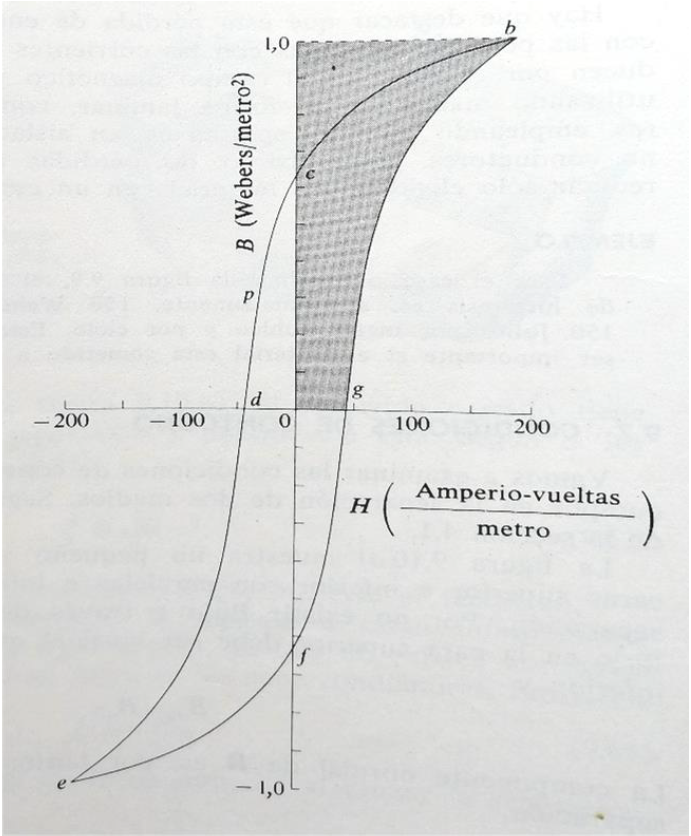
\includegraphics[scale=0.5]{histeresis.png}
    \caption{ciclo histéresis}
\end{figure}

\subsection{Energía de interacción de un dipolo en un campo magnético}

Como ya sabemos la energía total del sistema no es lo mismo que la energía magnética (por ejemplo para casos a $I$ constante tenemos que $U_T = - U_m$). Como nosotros entendemos un dipolo eléctrico como una espira muy pequeño podemos intuir que la energía del dipolo va con un signo menos. Si lo que queremos es conocer esa energía de interacción entre el dipolo y un campo magnético de manera explícita tenemos que deducir la expresión de otra manera. \\

El desarrollo matemático para llegar a la expresión final es bastante complicado y enredado, por ello escribiremos la expresión final directamente:

\begin{equation}
\vec{F}_m = \nabla (\vec{m} \cdot \vec{B}) 
\end{equation}
 
 \begin{equation}
 U_m = - \vec{m} \cdot \vec{B}
 \end{equation}
 
 
 \subsection{Energía almacenada en un material imanado}
 
 La energía que hay que aportar para imanar un campo viene dado por la ecuación:
 
 \begin{equation}
 \Delta W = \int \D \tau \vec{B}_0 \cdot \D \vec{M}
 \end{equation}

suponiendo que inicialmente existe un campo $\vec{B}_0$.
\newpage

\section{Ecuaciones de Maxwell: vector de Poynting}

Maxwell formulo en 1861 las conocidas como ahora leyes de Maxwell (que eran 13, luego Heavside las acorto en las 4 que son famosas). Antes que el la mayoría de estas leyes ya eran conocidas (ley de inducción de Faraday, ley de Gauss, ley de Ampére...) sin embargo fue el quien las unió y añadió un término que las completaba, creando la conocida ley de Ampére-Maxwell. De hecho el término que añadió le permitió deducir que la luz no era mas que una onda electromagnético, hecho que se demostraría posteriormente. Las ecuaciones de maxwell son, en formulación diferencial: \\

\begin{equation}
\begin{array}{lll}
\nabla \cdot \vec{E} & = & \dfrac{\rho_v}{\varepsilon_0} \\ 

\nabla \times \vec{E} & = & - \dfrac{\partial \vec{B}}{\partial t} \\ \\

\nabla \cdot \vec{B} & = & 0 \\ 

\nabla \times \vec{B} & = & \mu_0 \vec{J} + \mu_0 \varepsilon_0 \parentesis{\dfrac{\partial \vec{E}}{\partial t}}

\end{array}
\end{equation}

siendo el último término de la cuarta ecuación la aportación de Maxwell. Este se fijo que en la ecuación de Ampére faltaba un término que incluyese corrientes no estacionarias. Las corrientes no estacionarias aparecen cuando por ejemplo se cargan las placas de un condensador, ya que existe una acumulación de carga, regida por la ecuación de continuidad. \\

En el caso de un medio material con polarización y magnetización las leyes de Maxwell se pueden reescribir como:


\begin{equation}
\begin{array}{lll}
\nabla \cdot \vec{D} & = & \rho_{fv} \\ 

\nabla \times \vec{E} & = & - \dfrac{\partial \vec{B}}{\partial t} \\ \\

\nabla \cdot \vec{B} & = & 0 \\ 

\nabla \times \vec{H} & = &  \vec{J_f} + \parentesis{\dfrac{\partial \vec{D}}{\partial t}}

\end{array}
\end{equation}

De la segunda ley de maxwell podemos deducir que $\rota E = \parciales{}{t} \parentesis{\rota A}$, por lo que $E = \parciales{A}{t}$. Sin embargo esto es falso, ya que $\vec{E}$ puede venir dado también por el gradiente de un potencial, ya que al hacer el rotacional del gradiente será cero. Entonces:

\begin{equation}
\vec{E} = -  \nabla V - \parciales{\vec{A}}{t} ; \tquad \vec{B} = \rota \vec{A}
\end{equation}

Sin embargo ya hemos dicho que este potencial es arbitrario. Lo único que debe verificarse siempre es que la divergencia de $\vec{E}$ tiene que ser igual a la densidad de carga, de tal forma que:

\begin{equation}
-\nabla^2 V - \dive \parentesis{\parciales{\vec{A}}{t}} = \dfrac{\rho}{\varepsilon_0}
\end{equation}

Llamamos como \textbf{gauge de Lorenz} a la condición $\dive \vec{A} = 0$, de tal manera que se verifique la siguiente condición. $$\nabla^2 V = \dfrac{\rho}{\varepsilon_0}$$ Esta es la única forma para la cual se verifican los potenciales que se trasmiten como ondas. Si no encontramos una elección particular que satisfaga la condición de Lorenz tenemos que encontrar una que si lo haga, pudiendo redefinir un nuevo potencial que si lo haga y si se trasmita como una onda.


\subsection{Condiciones de frontera}

Sabemos que los campos $\vec{E}, \vec{D}, \vec{B}, \vec{H}$ serán discontinuos en las superficies de separación de dos medios diferentes, en una superficie que tenga densidad de carga $\sigma$ o una densidad superficial de carga $\vec{k}$. Podemos deducir explícitamente estas discontinuidades de las ecuaciones de Maxwell en forma  integral:


\begin{equation}
\oint_S \vec{D} \cdot \D \vec{A} =  Q_{f_{enc}} \label{Ec:6.1-1EcMaxInt}
\end{equation}
\begin{equation}
\oint_S \vec{B} \cdot \D \vec{A} =  0  \label{Ec:6.1-2EcMaxInt}
\end{equation}
\begin{equation}
\oint_S \vec{E} \cdot \D \vec{l} =  - \dfrac{\D }{\D t} \int_S \vec{B} \D \vec{A} \label{Ec:6.1-3EcMaxInt}
\end{equation}
\begin{equation}
\oint_c \vec{H} \cdot \D \vec{l} =  I_{f_{enc}} +  \dfrac{\D }{\D t} \int_S \vec{D}\label{Ec:6.1-4EcMaxInt} \D \vec{A}
\end{equation}

\begin{figure}[h!] \centering
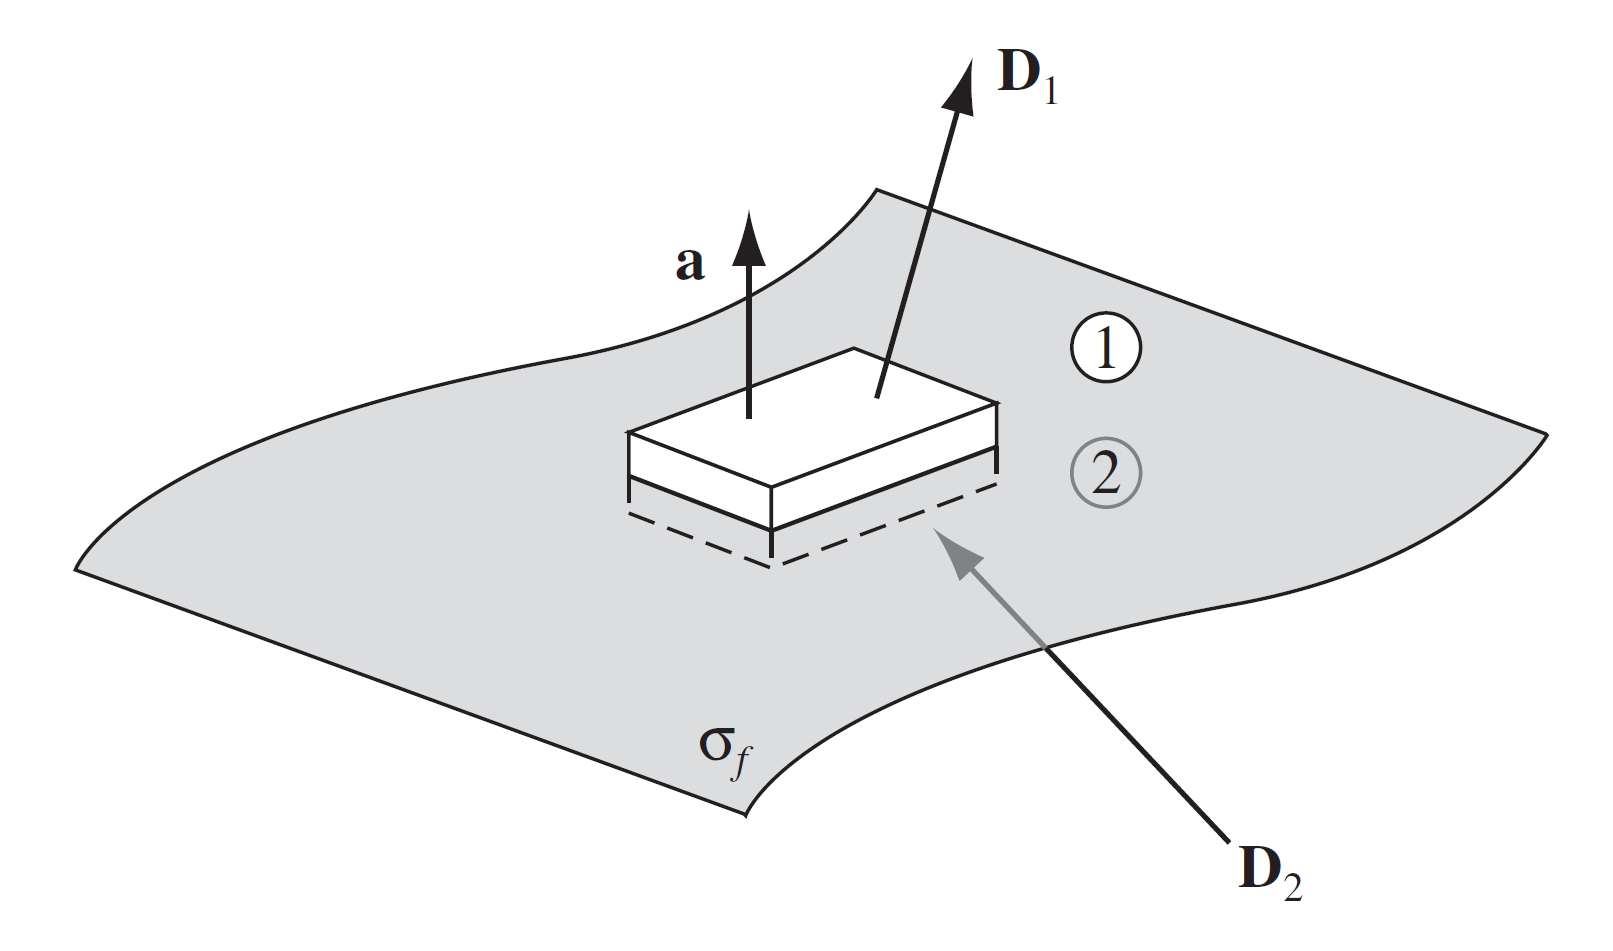
\includegraphics[scale=0.3]{condicionesmaxwell1.png}
\label{Fig:6.1}
\caption{volumen gaussiano}
\end{figure}



\begin{figure}[h!] \centering
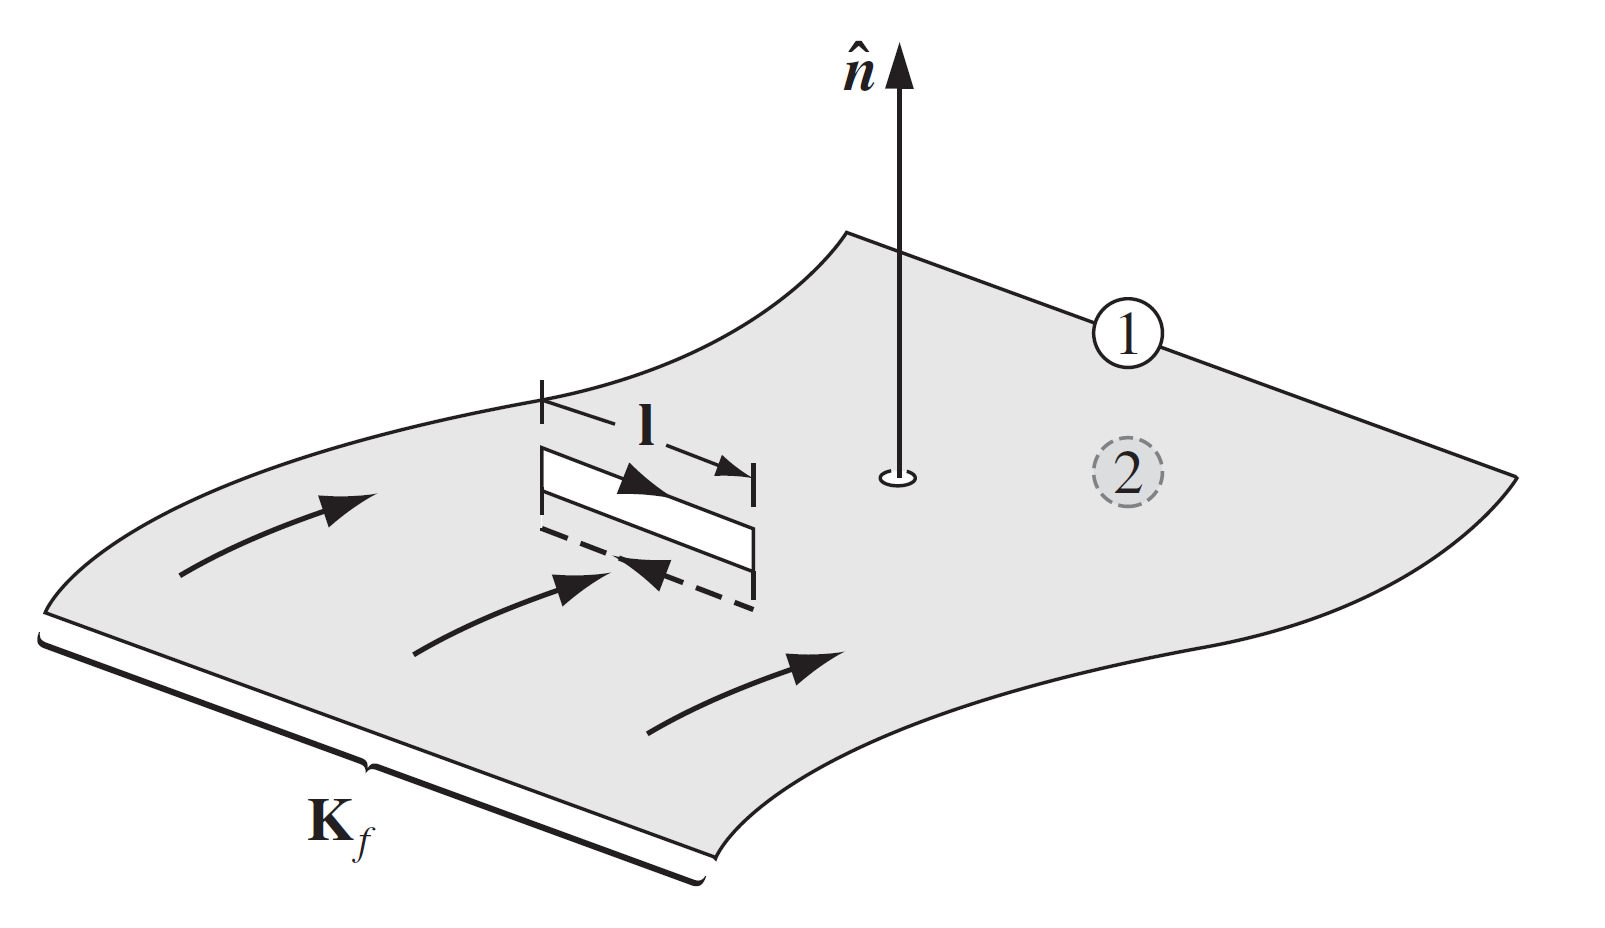
\includegraphics[scale=0.3]{condicionesmaxwell2.png}
\label{Fig:6.2}
\caption{curva amperiana}
\end{figure}

Si aplicamos la ecuación \ref{Ec:6.1-1EcMaxInt} y la ecuación \ref{Ec:6.1-2EcMaxInt} a un pequeño volumen gaussiano como el de la figura \ref{Fig:6.1}, obtenemos que:

\begin{equation}
D_{1n} - D_{2n} = \sigma_f
\end{equation}

\begin{equation}
B_{1n} - B_{2n} = 0
\end{equation}

Ahora aplicamos para la ecuación \ref{Ec:6.1-3EcMaxInt} y \ref{Ec:6.1-4EcMaxInt} una pequeña curva amperiana de tal manera que la superficie de separación quede entre ellas. En el caso de la ecuación \ref{Ec:6.1-3EcMaxInt} tenemos que en la curva:

$$ \vec{E_1} \cdot \vec{l} - \vec{E_2} \cdot \vec{l} = - \dfrac{\D}{\D t} \int_S \vec{B} \D \vec{A} $$

pero en el límite cuando la altura de la curva tiende acero el flujo desaparece, ya que disminuye la superficie pero no aumenta el campo lo suficiente para mantener constante. Entonces:

\begin{equation}
\vec{E_{1t}} - \vec{E_{2t}} = 0
\end{equation}

Es decir las componentes tangenciales se conservan (paralelas a la superficie, usando la expresión del Grifftiths). Lo mismo aplica a la ecuación \ref{Ec:6.1-4EcMaxInt} y figura \ref{Fig:6.2} ya que la integral de superficie de $\vec{D}$ también tiende a cero cuando la altura se reduce.:

\begin{equation}
\vec{H}_{1t} - \vec{H}_{2t} = \vec{K}_f \times \vec{n}
\end{equation}

en particular estas ecuaciones se pueden expresar facilmente en términos de $\vec{E} $ y $\vec{B}$ si el medio es lineal (l.h.i).


\subsection{Ecuaciones de propagación de los campos}

Partiendo de las ecuaciones de maxwell podemos deducir las ecuaciones de propagación del los campos. Si hacemos el rotacional del rotacional de $\vec{E}$ tenemos que:

$$
\nabla (\nabla \cdot \vec{E}) -  \nabla^2 \vec{E} = \mu_0 \vec{J} + \mu_0 \varepsilon_0 \pparciales{\vec{E}}{t} \Longrightarrow
$$

\begin{equation}
\nabla^2 \vec{E} -  \mu_0 \varepsilon_0 \pparciales{\vec{E}}{t}  = \dfrac{\nabla \rho_v}{\varepsilon} + \mu_0 \vec{J}
\end{equation}
que si estamos lo suficientemente lejos de las fuentes podemos llegar a que:

\begin{equation}
\nabla^2 \vec{E} -  \mu_0 \varepsilon_0 \pparciales{\vec{E}}{t}  = 0
\end{equation}
que no es otra cosa que una ecuación de ondas. A esta ecuación se le llama la \textit{ecuación de propagación de ondas del campo} $\vec{E}$. La velocidad de propagación sería $1/v^2 = \mu_0 \varepsilon_0$. Podemos estudiar lo mismo para el campo $\vec{B}$ llegando a que:


\begin{equation}
\nabla^2 \vec{B} -  \mu_0 \varepsilon_0 \pparciales{\vec{E}}{t}  = \mu_0 \nabla \times \vec{J} \Longrightarrow
\end{equation}
\begin{equation}
\nabla^2 \vec{B} -  \mu_0 \varepsilon_0 \pparciales{\vec{B}}{t}  = 0
\end{equation}
que es la respectiva \textit{ecuación de propagación de ondas del campo} $\vec{B}$, con la misma velocidad Maxwell. Lo que le hizo sospechar a Maxwell de que la luz era una forma de radiación electromagnética fue que $v_p = 3 \cdot10^8 \ m/s$, muy similar a la velocidad de la luz, proponiendo que la luz era radiación electromagnético. De esta forma Maxwell unifico la electricidad, el magnetismo y la óptica. Los potenciales también se trasmiten como ondas, siempre que se verifique la \textit{condición de Lorenz} (satisfaciendo los potenciales el \textit{gauge de Lorenz}):

\begin{equation}
\nabla^2 \vec{A} -  \mu_0 \varepsilon_0 \pparciales{\vec{a}}{t}  = - \mu_0 \vec{J}; \tquad 
\nabla^2 \vec{V} -  \mu_0 \varepsilon_0 \pparciales{\vec{V}}{t}  = - \dfrac{\rho}{\varepsilon_0}
\end{equation} 

Sin embargo no es suficiente que las ecuaciones de onda se satisfagan, también deben verificarse las ecuaciones de Maxwell (para definir completamente $\vec{E}$ y $\vec{B}$. Las ecuaciones de onda son consecuencias de las ecuaciones de Maxwell, y al resolverse las primeras se debe tener en cuenta que tienen que verificar estas últimas. Al obtener las ecuaciones a partir del rotacional del rotacional de las leyes de Maxwell se pierde información.







\subsubsection{Variación temporal armónica}
En general nosotros prestaremos atención sobretodo a las ondas sinusoidales, ya que si algo vibra en general la ecuación del oscilador armónico siempre va a estar presente, prácticamente en cualquier campo de la física. A veces estará mas decorada, pero en general las soluciones tendrán, con total certeza, relación con el oscilador armónico. Por eso vamos a considerar que las ondas son sinuisoidales. (Nota: aunque no lo fuera cualquier perturbación periódica se puede escribir como la suma de senos y cosenos por los desarrollos de Fourier).\\

Denominamos \textbf{fasor vectorial} a una forma de representar un el movimiento sinuisoidal de un campo cualquiera. Se representa así porque es mas cómodo trabajar en números complejos (sobretodo cuando se trata de sumar o multiplicar diferentes ondas). En general lo representamos como:

\begin{equation}
\vec{E} (\vec{r},t) = \mathrm{Re} \left[ \vec{E} (\vec{r},t) e^{jwt} \right] = \vec{E} (\vec{r}) \cos (wt)
\end{equation}
si esto es así la ecuación de las ondas se transforma en:

\begin{equation}
\nabla^2 \vec{E} (\vec{r}) + \dfrac{w^2}{c^2} \vec{E} (\vec{r}) = 0
\end{equation}

y por lo tanto el número de onda $k = w/c$ y $\lambda = 2 \pi/k$, llamando a $\lambda$ a la longitud de onda. El \textbf{número de onda} $k$ dependerá de la frecuencia ($w$) y las características del medio ($v_p \neq c$). \\


Supongamos primero que nuestros campos tienen la dirección $\widehat{z}$, sin ningún tipo de dependencia en $x$ e $y$ (en la propagación). Estas ondas son llamas \textbf{ondas planas} porque la vibración de los campos se encuentra encerrada en un plano perpendicular a la dirección de propagación. Una onda que se propague en la dirección $z$ como nuestros campos se podrán escribir como

\begin{equation}
\vec{E}(z,t) = \vec{E_0} e^{i(kz-wt)}; \tquad
\vec{B}(z,t) = \vec{B_0} e^{i(kz-wt)}
\end{equation}


Debido a que la divergencia de ambos campos será cero (si estamos lejos de las fuentes escalares del campo eléctrico) tenemos que el término que va con $z$ de $\vec{E_0}$ y $\vec{B_0}$ tiene que ser nulo. Además tenemos en cuenta por la ecuación que $E \perp B$. En general consideraremos la dirección de $\vec{E}$ para especificar como se dirigen los vectores. Si suponemos que $\vec{E_0} = E_0 \widehat{n}$ tenemos que:

$$
\nabla \times \vec{E} = - \dfrac{\partial \vec{B}}{\partial t} \Longrightarrow \vec{B_0} = \dfrac{k}{w} (\widehat{z} \times \vec{E_0}) = \dfrac{1}{c} (\widehat{z} \times \vec{E_0})
$$

\begin{figure}[h!] \centering
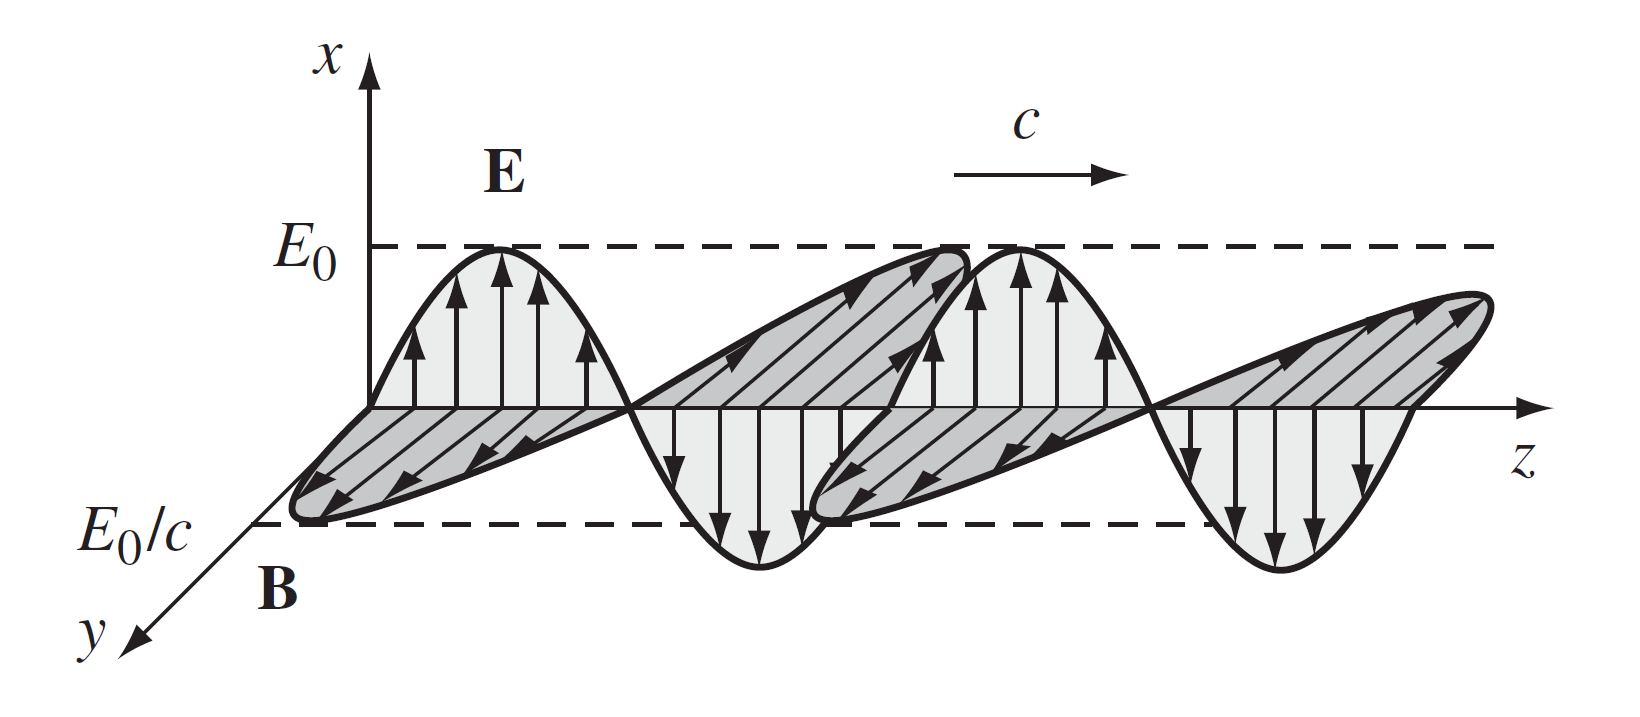
\includegraphics[scale=0.4]{ondaselectromagneticas.png}
\caption{Propagación de una onda en el espacio, con $\vec{k} || \widehat{z}$}
\end{figure}

Esta claro que la elección de propagación sobre el eje $z$ es completamente arbitrario: podemos generalizar el movimiento de una onda electromagnética a través de cualquier dirección. Para esto lo que hacemos es definir un vector $\vec{k}$ \textit{normalizado} que será el \textbf{vector de onda} o \textbf{vector de propagación}. Entonces ahora si $\vec{r}$ es el vector posición de un punto cualquiera:

\begin{equation}
\vec{E}(r,t) = \vec{E_0} e^{i (\vec{k}\cdot \vec{r} + wt)} \widehat{n}; \tquad \vec{B}(r,t) = \dfrac{1}{c} E_0 e^{i (\vec{k} \cdot \vec{r} + wt)} (\widehat{k} \times \widehat{n})
\end{equation}
llamamos al vector $\widehat{n}$ el \textbf{vector de polarización}.

\subsubsection{Potenciales retardados:}

Hemos visto que los campos electromagnéticos se propagan a una velocidad (por el vacío) de $v_p = c = 1/\sqrt{\varepsilon_0 \mu_0}$ (para un medio l.h.i. $v_p = 1/\sqrt{\varepsilon_0 \mu_0}$). Por lo tanto el campo en un punto vendrá dado por unas fuentes cuyos efectos tardan un tiempo en llegar a ese punto.  El tiempo que tardará en llegar de $\vec{r'}$ a $\vec{r}$ desde la fuente será de $t = R/v_p$, donde $R = |\vec{r}-\vec{r}'|$. Es evidente que tiene que ser así: a menor velocidad mas tiempo va a tardar en llegar la señal. Si no fuera así en todo el espacio aparecería la misma señal, sin distinguir el punto del espacio . Entonces el potencial escalar eléctrico (para el potencial vectorial magnético se hace de manera análoga):

\begin{equation}
V(\vec{r},t) = \dfrac{1}{4 \pi \varepsilon_0} \int_{V'} \dfrac{\rho (\vec{r},t-R/v_p)}{|\vec{r}- \vec{r'}}| \ \D \tau
\end{equation}

En el caso de que $v_p \rightarrow \infty$ tendríamos que la señal sería instantánea. Sin embargo sabemos que no es así. El potencial escalar magnético también se retarda:

\begin{equation}
\vec{A} (\vec{r},t) = \dfrac{\mu}{4 \pi} \int_{V'} \dfrac{\vec{J}(\vec{r},t-R/v_p)}{|\vec{r}- \vec{r}'|} \ \D \tau
\end{equation} 

Si consideramos el caso armónico tenemos que la variación temporal vendrá dada por:

\begin{equation}
V(\vec{r},t) = \dfrac{1}{4 \pi \varepsilon_0} \int_{V'} \dfrac{\rho_v \  e^{jw(t-R/v_p)}}{|\vec{r}-\vec{r'}|} \ \D \tau
\end{equation}
\begin{equation}
\vec{A}(\vec{r},t) = \dfrac{1}{4 \pi \varepsilon_0} \int_{V'} \dfrac{\vec{J} \  e^{jw(t-R/v_p)}}{|\vec{r}-\vec{r'}|} \ \D \tau
\end{equation}


para que en un tiempo cualquiera no exista retraso (o prácticamente no haya retraso) en una región tenemos que la exponencial debe ser uno. Para esto:

$$wR/c \ll 1 \Longrightarrow R \ll c/w $$ 

Por ejemplo si ponemos una onda de frecuencia de 10 $kHz$ tenemos que $R \ll 5 km$, pero para ondas de $10 GHz$ tenemos que $R \ll 5 mm$. Si queremos hacer aproximaciones cuasiestáticas para frecuencias muy grandes tenemos que tener unas dimensiones espaciales pequeñas.

\subsubsection{Polarización de ondas planas}

La polarización de una onda plana uniforme describe el comportamiento de $\vec{E}$ al variar el tiempo, en un punto determinado del espacio. Existen 3 tipos de polarización, y en este apartado vamos a estudiar cuales son. \\

La \textbf{polarización lineal} es la forma mas sencilla de todas. En esta polarización la onscilación solo se produce en una dirección, denotada como $x$ sin pérdida de generalidad. Un campo $\vec{E}$ linealmente polarizado se suele representar como:

$$ \vec{E} = E_0 \widehat{x} $$

La \textbf{polarización circular} viene dada por una oscilación en dos direcciones, con una desfasada respecto la otra en $\pi/2$, pero con una amplitud igual en ambas direcciones. Viene dada por:

$$ \vec{E} = \vec{x} E_0 \cos (kx-wt + \phi_0) + \vec{y} E_0 \sin (kx-wt + \phi_0) $$

Ademas diferenciamos las polarizaciones circulares \textbf{derechas} y las polarizaciones a \textbf{izquierdas}. La diferencia es que si está a derechas uno de las direcciones estará desfasada $-\pi/2$ y si esta desfasada $\pi/2$ tendremos que lo estará a izquierdas.  \\


La \textbf{polarización elíptica} es igual que la circular solo que las amplitudes en ambas direcciones son diferentes, además de que el desfase no tiene porque ser de $\pi/2$. 


$$ \vec{E} = \vec{x} E_1 \cos (kx-wt) + \vec{y} E_2 \cos (kx-wt+\delta) $$



\subsection{Energía y momento en ondas electromagnéticas}

Como sabemos, en un medio con campos eléctricos y campos magnéticos habrá una energía que vendrá dada por:

$$
U = \varepsilon_0 \int_V E^2 \D \tau +   \dfrac{1}{\mu_0} \int_V B^2 \D \tau
$$
por lo tanto la energía por unidad de volumen vendrá dada por: 

\begin{equation}
u = \varepsilon_0 E^2 + \dfrac{1}{\mu_0} B^2
\end{equation}

en el caso de que los campos tengan relación con una onda electromagnética tenemos que $B^2 = \mu_0 \varepsilon_0 E^2$, y entonces podemos decir que:

\begin{equation}
u = \varepsilon_0 E^2 = \varepsilon_0 E_0^2 \cos^2 (\vec{k} \vec{r} - wt + \delta)
\end{equation}

dado que la energía se propagará en la misma dirección que la onda. Dado que $E$ y $B$ son perpendiculares, podemos crear un vector llamado el \textbf{vector de Poyting} tal que:

\begin{equation}
\vec{S} = \dfrac{1}{\mu_0} (\vec{E} \times \vec{B})
\end{equation}

que se relaciona con la energía por unidad de volumen (asignando sin pérdida de generalidad un vector dirección $z$):

\begin{equation}
\vec{S} = c u \vec{z}
\end{equation}

que al igual que cuando hacíamos $\vec{J}=\rho_V \vec{v}$ tenemos la densidad de flujo de carga, en este caso el vector $S$ será la densidad de flujo de energía de una onda electromagnética. Para entenderlo mejor supongamos que en un tiempo $\Delta t$, una longitud $c \Delta t$ pasará a través de una área $A$ llevando consigo una energía $u A c \Delta t$. Es decir, la energía trasportada por unidad de área y tiempo será $c u$.\\


\begin{figure}[h!] \centering
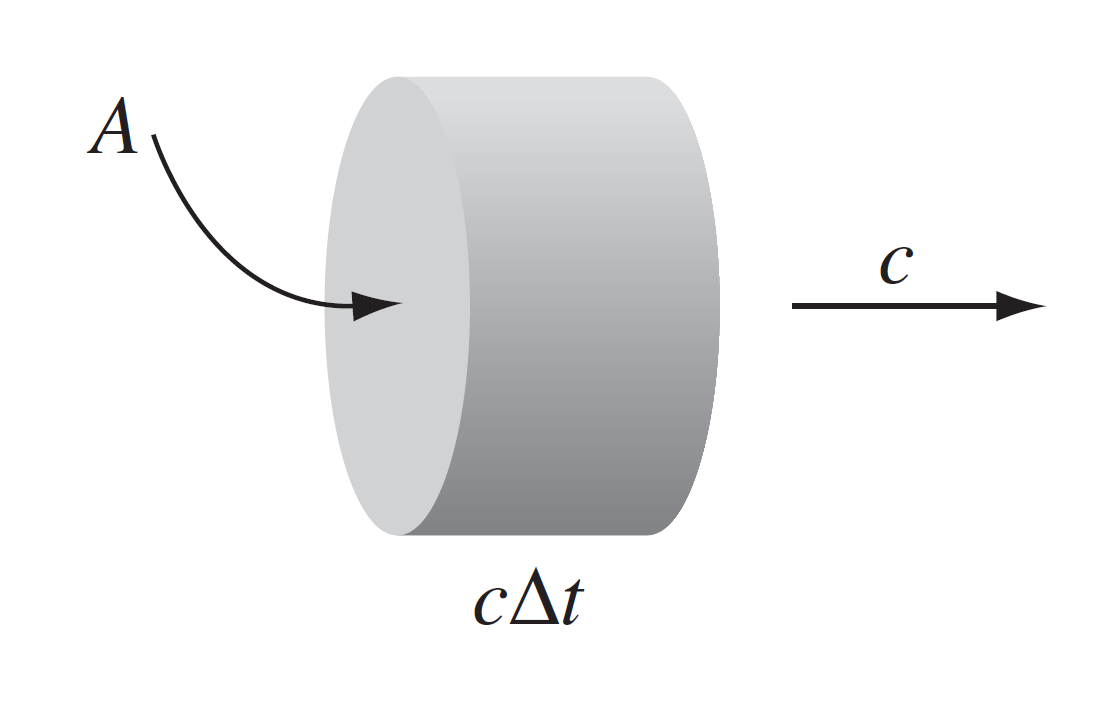
\includegraphics[scale=0.4]{densidadenergia.png}
\caption{flujo de energía}
\end{figure}

Además de trasportar energía, las ondas electromagnéticas (y por lo tanto los campos) transportan momento. De hecho la densidad de momento trasportado viene dado por:

\begin{equation}
\vec{g} = \dfrac{1}{c^2} \vec{S}
\end{equation}



\subsubsection{Promedios temporales}

Normalmente no estamos interesados en las fluctuaciones concretas seno-coseno en términos de densidad de energía y momento, si no que lo que queremos es el valor medio. Es mucho mas significativo conocer cual es el valor medio de la energía (o de la densidad de energía) en una región del espacio, más que nada porque si tenemos frecuencias muy altas el cálculo se complica. El valor medio de una función seno-coseno al cuadrado es de un medio $\langle \cos^2 (x) \rangle = 1/2$, por lo que solemos denotar como valores medios:

\begin{equation}
\begin{array}{lll}

\langle u \rangle & = & \dfrac{1}{2} \varepsilon_0  E_0 ^2 \\ \\

\langle \vec{S} \rangle & = & \dfrac{1}{2} c \varepsilon_0  E_0 ^2 \widehat{z} \\ \\

\langle \vec{g} \rangle & = & \dfrac{1}{2c} \varepsilon_0  E_0 ^2 \widehat{z}
 

\end{array}
\end{equation}

También se denota al valor medio de $S$ como la intensidad $I$, ya que es la energía por unidad de área trasportada por una onda. Cuando una onda electromagnética incide en un material que absorbe toda la onda tenemos que entrega momento a la superficie. En un tiempo $\Delta t$, el momento que se trasfiere viene dado por:

\begin{equation}
\Delta \vec{p} = \langle \vec{g} \rangle A c \delta t
\end{equation} 

por lo que la presión será:

\begin{equation}
P = \dfrac{1}{A} \dfrac{\Delta p}{\Delta t} (1+r) = \dfrac{I}{c} (1+r) = \dfrac{\langle \vec{S} \rangle}{c} (1+r) 
\end{equation}

Cualitativamente la presión magnética tiene un significado claro: el campo eléctrico mueve las cargas en su dirección, y una vez que adquieren velocidad el campo magnético debido a la fuerza de Lorentz moverá las cargas perpendicularmente a $\vec{B}$ y $\vec{E}$. La fuerza neta de todas las cargas es lo que ejerce la presión. El valor $r$ es una medida de la reflexión, tal que:

\begin{itemize}
\item $r=1$: 100\% reflexión.
\item $r=0$: absorción total.
\item $r=-1$: 100\% trasparencia.
\end{itemize}

Existe un teorema muy útil que nos dice que si $f=f_0 \cdot e^{jwt}$ y si $g = g_0 \cdot e^{jwt}$ tenemos que:

\begin{equation}
\langle \Real (f) \cdot \Real (g) \rangle = \dfrac{1}{2} \Real (f \cdot g ^*)
\end{equation}
se puede aplicar al resultado anterior como:

\begin{equation}
\langle \vec{S} \rangle = \dfrac{1}{2} \dfrac{1}{\mu_0} \Real (\vec{E} \times \vec{B}^* ) = \dfrac{1}{2} \Real (\vec{E} \times \vec{H}^*) 
\end{equation}

\subsection{Teorema de Poyting}

El teorema de Poyting nos dice como se relaciona la energía eletromagnética y el flujo de la energía con la realización de trabajo sobre las cargas. Como sabemos la fuerza que se ejerce sobre las cargas será $F = q(E+vB)$, y como el campo magnético no realiza trabajo tenemos que:

$$ \d W = \vec{F} \D \vec{l} = q \vec{E} \vec{v} \D t = \rho \D \tau \vec{E}  \vec{v} \D t  \Longrightarrow \dfrac{\D W}{\D t} = \vec{E} \cdot \vec{J} \D \tau \Longrightarrow$$

\begin{equation}
\dfrac{\D W}{\D t} = \int_V (\vec{E} \cdot \vec{J}) \D \tau \label{Ec:6.3.Trabajo}
\end{equation}

Ahora viene un desarrollo un tanto complicado, ya que lo que vamos a hacer es usar las ecuaciones de Maxwell para despejar $\vec{J}$ en función del rotacional de $B$ y la derivada temporal de $E$:

$$ \vec{J} = \dfrac{\nabla \times \vec{B}}{\mu_0} - \varepsilon_0 \parciales{\vec{E}}{t} \Longrightarrow \vec{E} \cdot \vec{J} = \vec{E} \cdot \parentesis{\dfrac{\nabla \times \vec{B}}{\mu_0} - \varepsilon_0 \parciales{\vec{E}}{t} }  $$
usamos la relación $\nabla \cdot (\vec{E} \times \vec{B}) = \vec{B} \cdot (\nabla \times \vec{E}) +  \vec{E} \cdot (\nabla \times \vec{B})$:

$$ \vec{E} \cdot \vec{J} = \dfrac{1}{\mu_0} \left[ \vec{B} \cdot (\nabla \times \vec{E}) -  \nabla (\vec{E} \times \vec{B}) \right] - \varepsilon_0 \vec{E} \cdot \parciales{\vec{E}}{t} $$
considerando las ecuaciones de Maxwell y que $\vec{E} \cdot \parciales{\vec{E}}{t}  = \parciales{E^2}{t}$ (lo mismo para $B$) tenemos que:

$$ \dfrac{\D W}{\D t} = \int_V \vec{E} \cdot \vec{J} = \parciales{}{t} \int_V \parentesis{\dfrac{1}{2 \mu_0} B^2 +  \dfrac{\varepsilon}{2}} E^2  - \mu_0 \oint_S (\vec{E} \times \vec{B}) \D \vec{A} $$
usando el vector de Poyting podemos enunciar el \textbf{teorema de Poyting} como:

\begin{equation}
\dfrac{\D W}{\D t} = - \dfrac{\D U_{em}}{\D t} - \oint_S \vec{S} \cdot \D \vec{A}
\end{equation} 

Es decir tenemos que cuando se realiza trabajo sobre las cargas por la fuerza electromagnética esta se manifiesta como una reducción de la energía almacenada por los campos menos la energía que fluye a través de la superficie, que viene dado por el flujo de energía $\vec{S}$. Entonces si $\D W = \int_V u_{mec} \D \tau$, tenemos que se puede expresar como:

\begin{equation}
\parciales{}{t} (U_{mec} + U_{em}) = - \int_V  (\nabla \cdot \vec{S}) \D \tau \longrightarrow \parciales{}{t} (u_{mec} + u_{em}) = - \nabla \cdot \vec{S}
\end{equation}

El significado de esta ecuación se descubre por si solo: la variación energía total en el sistema es positiva si y solo si el vector $S$ es antiparalelo al vector normal de la superficie, es decir, si el flujo de energía converge en esa superficie. Es una ecuación similar a la ecuación de continuidad de $\vec{J}$, ya que si y solo si $\nabla \cdot \vec{S}  = 0$ la energía dentro de una región es constante. En el caso de que haya materiales con permeabilidad y permitividad tenemos que la expresión es muy similar. \\

El trabajo dado por la ecuación \ref{Ec:6.3.Trabajo} puede entenderse como el \textit{efecto Joule} que ocurre al mover las cargas, ya que si existen portadores de carga su movimiento creará una dispersión de la energía en forma de calor. Entonces podemos entender el teorema de Poyting como la energía que se dispersa si llega un flujo de energía a un material con portadores de carga, como un conductor, aunque en este caso también se generarán corrientes superficiales. 

 

\subsection{Propagación en medios materiales}
 
Si el medio material es lineal homogéneo e isótropo y con conductividad, tenemos que en la presencia del campo eléctrico aparecerá una corriente tal que:

$$ \vec{J} = \sigma \vec{E} $$
 
por lo tanto cuando se trasmitan ondas electromagnéticas se trasmitirá también una corriente (si es un medio mínimamente conductor). Entonces las ecuaciones de Maxwell que aplicamos para deducir la ecuación de ondas son:

$$ \nabla \times \vec{E} = - \parciales{\vec{B}}{t}; \tquad \nabla \times \vec{B}  = \mu \varepsilon \parciales{\vec{E}}{t} + \mu \sigma \vec{E} $$

Eso nos lleva a deducir que:

\begin{equation}
\nabla^2 \vec{B} = \mu \sigma \parciales{\vec{B}}{t}  + \mu \varepsilon \parciales{^2 \vec{B}}{t^2}
\end{equation}
Supongamos ahora oscilaciones armónicas tal que:

$$ \vec{E} = E_0 e^{kz-wt}; \tquad \vec{B} = B_0 e^{kz-wt}; \tquad B_0 = E_0/v_p  $$
de tal forma que si tenemos una oscilación armónica la expresión será:

\begin{equation}
\nabla^2 \vec{B} = - (\mu \varepsilon w^2 + j \mu \sigma w) \vec{B} \label{Ec:6.5-79} 
\end{equation}

es decir una ecuación no homogénea. Ahora la velocidad de propagación depende de la frecuencia. Esto es lo que se conoce como ``medios dispersivos''. A veces definimos lo que se llama \textbf{permitividad compleja}, de tal forma que:

\begin{equation}
\varepsilon_c = \varepsilon - j \dfrac{\sigma}{w} \Longrightarrow = \varepsilon' + \varepsilon'' j
\end{equation}

\begin{equation}
\nabla^2 \vec{B} = \mu w^2 \varepsilon_c \vec{B}
\end{equation}
esto además permite relacionar el rotacional de $\vec{H}$ con $\vec{E}$:

$$ \rota \vec{H} = j w \varepsilon_c  \vec{E}$$

Definimos como \textbf{tangente de pérdidas} al cociente entre la parte imaginaria de la permitividad compleja y la parte real. Cuanto mayor sea esta relación obviamente las pérdidas serán mayores. Entonces:

\begin{equation}
\tan \delta_c = \dfrac{\varepsilon ''}{ \varepsilon ' } \cong \dfrac{\sigma}{w \varepsilon}
\end{equation} 
Ahora tenemos que calcular el número de onda, que se puede deducir al derivar respecto al laplaciano la ecuación \ref{Ec:6.5-79}, que ahora será un numero complejo:

\begin{equation}
k^2 = \mu \varepsilon w^2 + j \mu w \sigma \longrightarrow k = k' + k'' j
\end{equation}
Podemos calcular la parte real y la parte imaginaria como:

$$ k' = w \sqrt{\dfrac{\mu \varepsilon}{2}} \left[ \sqrt{1+\parentesis{\dfrac{\sigma}{\varepsilon w}}^2} +1 \right]^{1/2} $$

$$k'' = w \sqrt{\dfrac{\mu \varepsilon}{2}} \left[ \sqrt{1+\parentesis{\dfrac{\sigma}{\varepsilon w}}^2} -1 \right]^{1/2} $$
La solución a nuestro problema será:

\begin{equation}
\vec{E}(z,t) = E_0 e^{-k''x} e^{j(k'x-wt+\delta)}; \tquad
\vec{B}(z,t) = \dfrac{E_0 |k|}{w} e^{-k''x} e^{j(k'x-wt+\delta+\phi)}
\end{equation}
Si analizamos un poco los términos que nos salieron podemos entender un poco el problema. Obviamente aparecerá un desfase entre $E$ y $B$, ya que $k$ es un número complejo. Además aparece un término atenuador $e^{-k''z}$, llamando a $k''$ la \textit{constante de atenuación del medio}. Otra relación es:

\begin{equation}
E_0 = \dfrac{w \mu}{k} H_0 = \eta H_0
\end{equation} 
donde llamamos a $\eta$ la \textbf{impendancia de la onda} que es una característica compleja del medio. Como acabamos de ver el problema puede llegar a ser bastante grande, por eso generalizamos el problema en dos, para poder así hacer aproximaciones. Estos son las pequeñas pérdidas y el caso de los buenos conductores. Llamamos a $\delta$ a la \textbf{produndidad de penetración}, que es la cantidad de distancia que puede penetrar una onda en dicho medio. Es la inversa de $k''$, es decir, de la parte compleja de $k$. Muchas veces en este proceso en vez de usar el número de onda complejo usamos un factor llamado \textbf{constante de propagación de onda} de tal forma que:

\begin{equation}
\gamma = j k = \alpha + j \beta = j(k'+k''j)
\end{equation}

\begin{equation}
\alpha = - k''j; \quad  \beta = k'
\end{equation}

Podemos de esta forma obtener los valores de $\alpha$ y $\beta$ de tal forma que el campo eléctrico ahora vendrá dado por:

\begin{equation}
\vec{E} = \vec{E_0} e^{- \alpha z} \cdot e^{- j \beta z} e^{-wt} 
\end{equation}

En este caso el significado de $\alpha$ es el factor de atenuación, que exprea lo que se atenúa la amplitud cuando la onda avanza un metro; y $\beta$ es el factor de fase, ya que expresa la magnitud del cambio de fase que se produce cuando la onda viaja un metro. 

\subsubsection{Pequeñas pérdidas}

En este caso la conductividad $\sigma \ll w \varepsilon$. Entonces podemos expandir la raíz cuadrada compleja que queda al despejar $k$ en serie de Taylor de tal forma que $\sqrt{1+x} \approx 1+ \dfrac{1}{2} x - \dfrac{1}{8} x^2...$. Así la expresión para $k$ será:

\begin{equation}
k = w \sqrt{\mu \varepsilon} \left[ 1 + \dfrac{1}{2} \dfrac{\sigma}{w \varepsilon} j + \dfrac{1}{8} (\dfrac{\sigma}{w \varepsilon})^2 \right]
\end{equation}

De esta expresión podemos obtener tanto la velocidad de onda en dicho medio (velocidad de propagación) y la longitud de onda, además de tener la ecuación de $\vec{E}$ y $\vec{B}$.

\subsubsection{Buenos conductores}

En el caso de buenos conductores tendremos que $\sigma \gg w \varepsilon$. El número de onda será:

\begin{equation}
k \approx w \sqrt{\mu \varepsilon} \sqrt{\dfrac{j \sigma}{w \varepsilon}}
\end{equation}
Como conocemos el valor de $\sqrt{j} = e^{j \pi/4}$ obtenemos que en números complejos:

\begin{equation}
k = k' (1+j) \tquad k' = \sqrt{ \dfrac{w \mu \sigma }{2}}
\end{equation}

De esta expresión podemos obtener tanto la velocidad de onda en dicho medio (velocidad de propagación) y la longitud de onda, además de tener la ecuación de $\vec{E}$ y $\vec{B}$.
\newpage

\section{Circuitos}

En esta sección presentaremos la siguiente notación, para evitar confusiones o mal entendidos: las funciones variables en el tiempo se representan en minúscula ($v(t), i(t),p(t)$), las magnitudes constantes en mayúscula ($V,I,P$), y los valores máximos (amplitudes) con un subíndice $m$ en mayúscula ($V_m,I_m,P_m$). \\

En la teoría de circuitos usamos campos cuasi estacionarios, o estacionarios, que se propagan todos a la vez y no dependen de la posición del circuito. Para esto tenemos que restringir el tamaño del circuito. Para que sea válida la aproximación tenemos el tamaño del circuito tiene que ser mucho menor que la longitud de onda, es decir:


\begin{equation}
l_{max} \ll \frac{2 \pi c}{w}
\end{equation}


\subsection{Elementos del circuito}

Al suministrar energía eléctrica a un elemento pasivo de corriente este se comporta o responde de una o más de las tres formas que vamos a presentar. Si la energía se disipa decimos que el elemento es un \textit{resistivo} puro; si la almacena en un campo magnético decimos que es una \textit{bobina}  pura, y si la almacena en un campo eléctrico es un \textit{condensador} puro. En general un circuito contendrá los tres elementos mezclados de una u otra forma, aunque también es habitual que uno de los elementos predomine sobre los otros. Veamos ahora estos elementos:

\subsubsection{Resistencia}

La diferencia de potencial $v(t)$ entre dos terminales de un elemento resistivo puro es directamente proporcional a la intensidad de corriente $i(t)$. La constante de proporcionalidad se llama la \textbf{resistencia} eléctrica del elemento y se denota por una $R$. Se expresa como:

\begin{equation}
v(t) = R \cdot i(t) \ \ \ \ \ \  i(t) = \dfrac{v(t)}{R}
\end{equation}

La unidad de medida de la resistencia es el \textit{Ohmio} ($\Omega$). No se impone ningún tipo de restricción acerca de como debe ser la corriente: puede ser continua o alterna.\\

Si el voltaje o la intensidad vienen dadas por una onda sinusoidal podremos representarlo como fasores. En este caso $i(t)$ y $v(t)$ estarán en fase, con la misma frecuencia.
 
 
 
\subsubsection{Autoinducción}

Al variar con respecto al tiempo la corriente que circula por un circuito, el flujo magnético que lo atraviesa experimenta los mismos cambios. Ahora bien toda variación de flujo origina una fuerza electromotriz que se opone a dicha variación. En estas condiciones si por una bobina circula una corriente de intensidad variable se originará, la f.e.m. inducida será proporcional (si $\mu = \mathrm{cte}$) a la derivada de la intensidad respecto al tiempo. La constante de proporcionalidad $L$ se le llama \textbf{coeficiente de autoinducción} o \textbf{autoinducción}. Se expresa esta relación como:

\begin{equation}
v(t) = L \dfrac{\D i}{\D t} \ \ \ \ \ \ i(t) = \dfrac{1}{L} \int v(t) \D t
\end{equation}

La unidad de medida de la autoindcción son los \textit{Henries} ($H$). En este caso la corriente debe ser alterna para que se genere la respuesta, si $i(t)$ es constante no se producirá una respuesta de la bobina.  \\

Si el voltaje o la intensidad vienen dadas por ondas sinusoidales podemos representarlas como fasores. En este caso existirá un desfase entre las ondas, ya que si $v(t) = V_m e^{jwt}$ $I_m = V_m/L$ tenemos que $$i(t) = \dfrac{V_m e^{jwt}}{jwL} = \dfrac{I_m}{w} e^{j(wt-\pi/2)}$$ es decir existe un desfase, tal que $i(t)$ está desfasado $\pi/2$ de $v(t)$. 


\subsubsection{Capacidad}

La diferencia de potencial en bornes de un condensador es proporcional a la carga $q$ almacenada en él. La constante de proporcionalidad se llama \textbf{capacidad} del condensador. Dado que la intensidad que llega al condensador es igual a la carga que se acumula por unidad de tiempo tenemos que:

\begin{equation}
q(t) = C v(t); \ \ \ \ \ \ i(t) = \dfrac{\D  q(t)}{\D t} = \dfrac{\D v(t)}{\D t} \ \ \ \ \ \ v(t) = \dfrac{1}{C} \int i(t) \D t
\end{equation}

La unidad de mediad de la capacidad es \textit{Faradios}. Si el voltaje o la intensidad vienen dadas por ondas sinusoidales podemos representarlas como fasores. En este caso existirá un desfase entre las ondas, ya que si $v(t) = V_m e^{jwt}$ $I_m =C V_m$ tenemos que $$i(t) = jwCV_m e^{jwt} = w I_m e^{j(wt+\pi/2)}$$ es decir existe un desfase, tal que $v(t)$ está desfasado $\pi/2$ de $i(t)$.  



\subsection{Leyes de Kirchoff}

Las leyes de Kirchoff sirven para estudiar y resolver circuitos eléctricos, obteniendo así para una serie de generadores y elementos pasivos la diferencia de potencial entre cada uno de estos y la intensidad que circula por los mismos. De estas leyes de sigue el principio de superposición, necesario para calcular circuitos con generadores que generen señales a diferente frecuencia.

\subsubsection{Mallas}

En un circuito cerrado o malla la suma algebraica de las fuerzas electromotrices aplicadas (subidas de tensión) es igual a la suma de caídas de tensión en todos los elementos pasivos. En otras palabras: la suma de las diferencias de potencial en todo circuito cerrado es nula. No nos importa que consideramos subida o bajada, pero es importante decirlo y ser constante con la elección en todo el circuito. Es importante observar que los voltajes de los generadores han de sumarse según vaya de más a menos: podemos asignar fuentes positivas (negativas) las que su sentido de polaridades van de - a +, si luego las que van de + a - son negativas (positivas). \\

Es mucho mas sencillo entender que se hace viendo un ejemplo o como se resuelve un circuito por mallas, por ello traemos el siguiente ejemplo.

\subsubsection{Nudos}

En un circuito la suma de intensidades de corrientes que llegan a un nudo es igual a la suma de las intensidades que salen de él. SI se consideran positivas las corrientes que llegan y negativas las que salen, esta ley estableces que la suma algebraica de las intensidades de todas las corrientes que concurren en un nudo es cero. 


\subsection{Impedancia}

En general en un circuito no tendremos elementos puros, si no que mezclas de resistencias, de bobinas y de condensadores; conectados en serie y en paralelo. La impedancia es un factor que da cuenta de todas estas, y se calcula entre dos puntos como el cociente entre el voltaje y la intensidad entre dos puntos:

\begin{equation}
Z = \dfrac{v(t)}{i(t)}
\end{equation}

 Cuando tenemos ondas sinusoidales es muy sencillo de calcularlo, ya que tendrá una parte real y otra compleja. La parte real vendrá dada por la resistencia y la compleja dependerá de los condensadores y las bobinas. Además se sumarán y contarán como las resistencias: si tenemos un varias impedancias en paralelo:

\begin{equation}
\dfrac{1}{Z_T} = \dfrac{1}{Z_1} + \dfrac{1}{Z_2} + \cdots + \dfrac{1}{Z_n}
\end{equation}

y si están en serie:

\begin{equation}
Z_T = Z_1 + Z_2 + \ldots + Z_n
\end{equation}

Esto se puede deducir directamente de las leyes de Kirchoff. Vamos a suponer los ejemplos mas comunes de estos: los circuitos RL y RC en serie.  \\

\shadowbox{\textbf{Circuito RL}}

\hrulefill

Si tenemos un circuito donde un generador suministra una potencia $v(t) = V_m e^{iwt}$ donde cogemos la parte real (notación fasorial) tenemos que según la ley de Kirchoff:

\begin{equation}
V_m e^{jwt} = R I_m e^{iwt} + jwLI_m e^{iwt} 
\end{equation}

por lo que:



\begin{equation}
I_m = \dfrac{V_m}{R + jwL}
\end{equation}

de lo que se deduce que nuestra impedancia:

\begin{equation}
Z = R + jwL = |R^2 + w^2 L^2| e^{i \phi} \tquad \phi = \arctan(wL/R)
\end{equation}

y por lo tanto la intensidad lleva un desfase frente al voltaje

\hrulefill \\


\shadowbox{\textbf{Circuito RC}} 

\hrulefill 

Si tenemos un circuito donde un generador suministra una potencia $v(t) = V_m e^{iwt}$ donde cogemos la parte real (notación fasorial) tenemos que según la ley de Kirchoff:

\begin{equation}
V_m e^{jwt} = R I_m e^{iwt} + \dfrac{1}{jwC} e^{iwt} 
\end{equation}

por lo que:



\begin{equation}
I_m = \dfrac{V_m}{R +  \dfrac{1}{jwC}}
\end{equation}

de lo que se deduce que nuestra impedancia:

\begin{equation}
Z = R - \dfrac{j}{wC} = \left| R^2 +  \parentesis{\dfrac{1}{wC}}^2 \right| e^{i \phi} \tquad \phi = \arctan(-\dfrac{1}{wCR})
\end{equation}

y por lo tanto la intensidad lleva un desfase frente al voltaje.

\hrulefill \\

\shadowbox{\textbf{Circuito RLC}}

\hrulefill 

Si tenemos un circuito donde un generador suministra una potencia $v(t) = V_m e^{iwt}$ donde cogemos la parte real (notación fasorial) tenemos que según la ley de Kirchoff:

\begin{equation}
V_m e^{jwt} = R I_m e^{iwt} + \dfrac{1}{jwC} e^{iwt}  + jwLI_m e^{iwt}  
\end{equation}

por lo que:

\begin{equation}
I_m = \dfrac{V_m}{R +  \dfrac{1}{jwC} + jwL}
\end{equation}

de lo que se deduce que nuestra impedancia:

\begin{equation}
Z = R + j\parentesis{wL - \dfrac{1}{wC}}= \left| R^2 +  \parentesis{wL -\dfrac{1}{wC}}^2 \right| e^{i \phi} \tquad \phi = \arctan(\dfrac{wL  - 1/wC}{R})
\end{equation}

y por lo tanto la intensidad lleva un desfase frente al voltaje, a no ser que $1/wC = wL$ que entonces el desfase será cero. El valor de la frecuencia para el que ocurre esto se llama \textit{frecuencia de resonancia}, aunque ya lo estudiaremos mejor mas adelante.

\hrulefill \\


Como podemos comprobar en ambos ejemplos la impedancia es un número complejo, que podemos expresar de manera exponencial:

\begin{equation}
Z = |Z| e^{j\phi}
\end{equation}

Arriba hemos descrito la función en el dominio del tiempo, sin embargo podemos expresarlo en el dominio de la frecuencia, donde solo importan los módulos (en valores eficaces) y el desfase:

\begin{equation}
\dfrac{I_m}{\sqrt{2}} e^{j(\alpha - \theta)} = \dfrac{V_m}{\sqrt{2}} \dfrac{e^{j\alpha}}{z e^{j \theta}}
\end{equation}

Definimos \textbf{amictancia} $Y$ como la inversa de la impedancia.

\begin{equation}
Y = \dfrac{1}{Z}
\end{equation}

\subsection{Valor medio y eficaz}

En el análisis de circuitos solo estudiamos funciones periódicas, es decir aquellas en las que $f(t) = f(r+nT)$ donde $n$ es un número entero y $T$ el periodo, que es el inverso de la frecuencia. El valor medio de una función periódica ya lo hemos estudiado en la sección de ondas, promedios temporales. Sea $y(t)$ una función periódica $T$ por definición:

\begin{equation}
Y_{ef} = \dfrac{1}{T} \int_0^T y(t) \D t
\end{equation}

\subsubsection{Valor eficaz}

Al circular una corriente de intensidad $i(t)$ por un elemento resistivo puro este disipa una potencia $p(t)$ con un valor medio $P$. Pues bien esta misma potencia $P$ la puede disipar una corriente constante de intensidad $I$ circulando por dicha $R$. En estas condiciones diremos que $i(t)$ tiene un valor eficaz $I_{ef}$ equivalente a la corriente constante $I$. Lo mismo diríamos de la tensión eficaz $V_{ef}$. Entonces definimos el valor eficaz de una función $y(t)$ de periodo $T$ que viene dado por:

\begin{equation}
Y_{ef} = \sqrt{\dfrac{1}{T} \int_0^T (y(t)^2 \D t}
\end{equation}

el valor eficaz de una función $a \sin (wt)$ o $a \cos (wt)$ es $a/\sqrt{2}$.

\subsection{Teorema de Thevenin y Norton}

El teorema de Thevenin y el teorema de Norton son unos teoremas que nos permiten calcular las intensidades y voltajes entre dos puntos cualquiera del circuito (entre los cuales habrá una impedancia cualquiera) de manera sencilla sin tener que resolver todo el circuito por mallas o por nudos. De esta forma podremos reemplazar el circuito activo por un circuito simple equivalente. 

\subsubsection{Teorema de Thevenin}

El \textbf{teorema de Thevenin} establece que cualquier circuito lineal activo con terminales de salida A y B puede substituirse (o es equivalente) a una fuente de tensión $V'$ en serie con una impedancia $Z'$. \\

La \textit{tensión equivalente de Thevenin}, $V'$, es la tensión entre los terminales $AB$ medida a circuito abierto y la \textit{impedancia equivalente}, $Z'$, es la impedancia de entrada en los terminales $AB$ con todas las fuentes internas iguales a cero.

\subsubsection{Teorema de Norton}

El \textbf{teorema de Norton} establece que cualquier circuito lineal activo con terminales de salida $AB$ puede substituirse (es equivalente) a una fuente de intensidad $I'$ en paralelo con una impedancia $Z'$. \\

La \textit{fuente de intensidad} $I'$ \textit{equivalente de Norton} es la corriente en un cortocircuito aplicado a los terminales del circuito activo. La impedancia $Z'$ en paralelo es la impedancia de entrada del circuito en los terminales $AB$ cuando se hacen igual a cero todas las fuentes internas. Por consiguiente dado un circuito lineal activo las impedancias $Z'$ de los circuitos equivalentes Thevenin y Norton son idénticas. \\

La intensidad de la corriente en una impedancia conectada a los terminales del circuito equivalente de Norton ha de tener el mismo sentido que la que circularía por la misma impedancia conectada al circuito activo original.

\subsection{Potencia y factor potencia}

En muchos dispositivos eléctricos uno de los parámetros mas importantes es la potencia. La tensión aplicada a un circuito de elementos pasivos es una función del tiempo, ya que viene dada por:

\begin{equation}
p(t) = v(t) \cdot i(t)
\end{equation}

pudiendo ser positiva o negativa, positiva si \textit{la energía va de la fuente a la red}, y negativa si \textit{la energía va de la red a la fuente}. 


\subsubsection{Potencia activa}
Consideremos en primer lugar que las señales son sinusoidales, de tal forma que podramos escribir. Supongamos ahora un caso ideal con un circuito pasivo que contenga una bobina pura. Tenemos que la intensidad y el voltaje estarán desfasados (la intensidad está desfasada), por lo que: 

\begin{equation}
p_L(t) = I_m V_m \sin (w t) \sin (w t - \pi/2) = - I_m V_m \sin (wt) \cos(wt) = -\dfrac{1}{2} V_m I_m \sin (2 wt)
\end{equation}

Si $v$ e $i$ tienen el mismo signo la fuente estará enviando energía al elemento pasivo, pero si tienen signos contrarios será la bobina quien envíe energía. La bobina tendrá el doble de frecuencia que la intensidad y el voltaje. Además su valor medio en un ciclo es cero. Para un condensador ocurrirá exactamente lo mismo, ya que la intensidad esta adelantada $\pi/4$:

\begin{equation}
p_C (t) = \dfrac{1}{2} V_m I_m \sin (2wt)
\end{equation}
sin embargo para una potencia no, ya que no están desfasados. Tenemos pues que:

\begin{equation}
p_R (t) = V_m I_m \sin^2 (wt) 
\end{equation}

\begin{figure}[h!] \centering
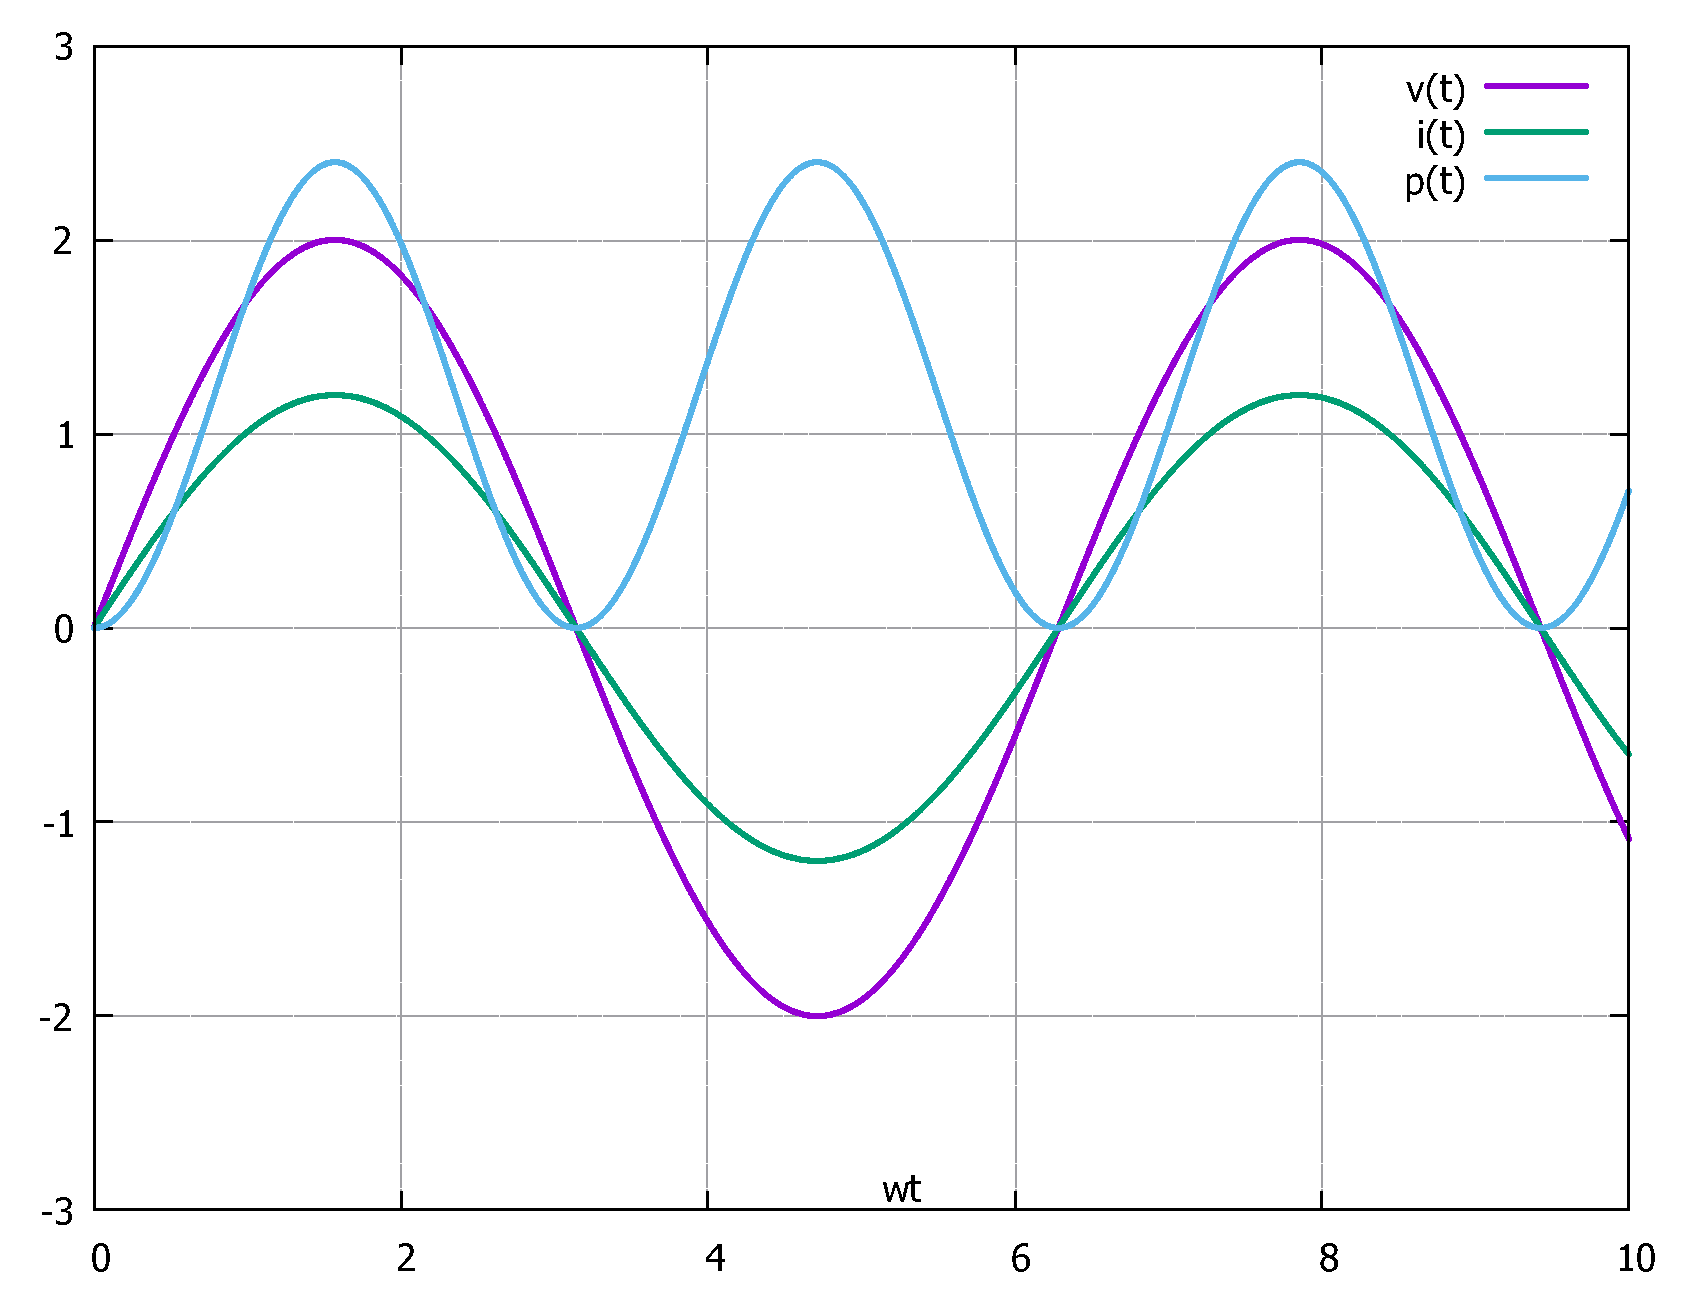
\includegraphics[scale=0.3]{potenciaresistencia.pdf}
\caption{Potencia a través de una resistencia pura}
\end{figure}

\begin{figure}[h!] \centering
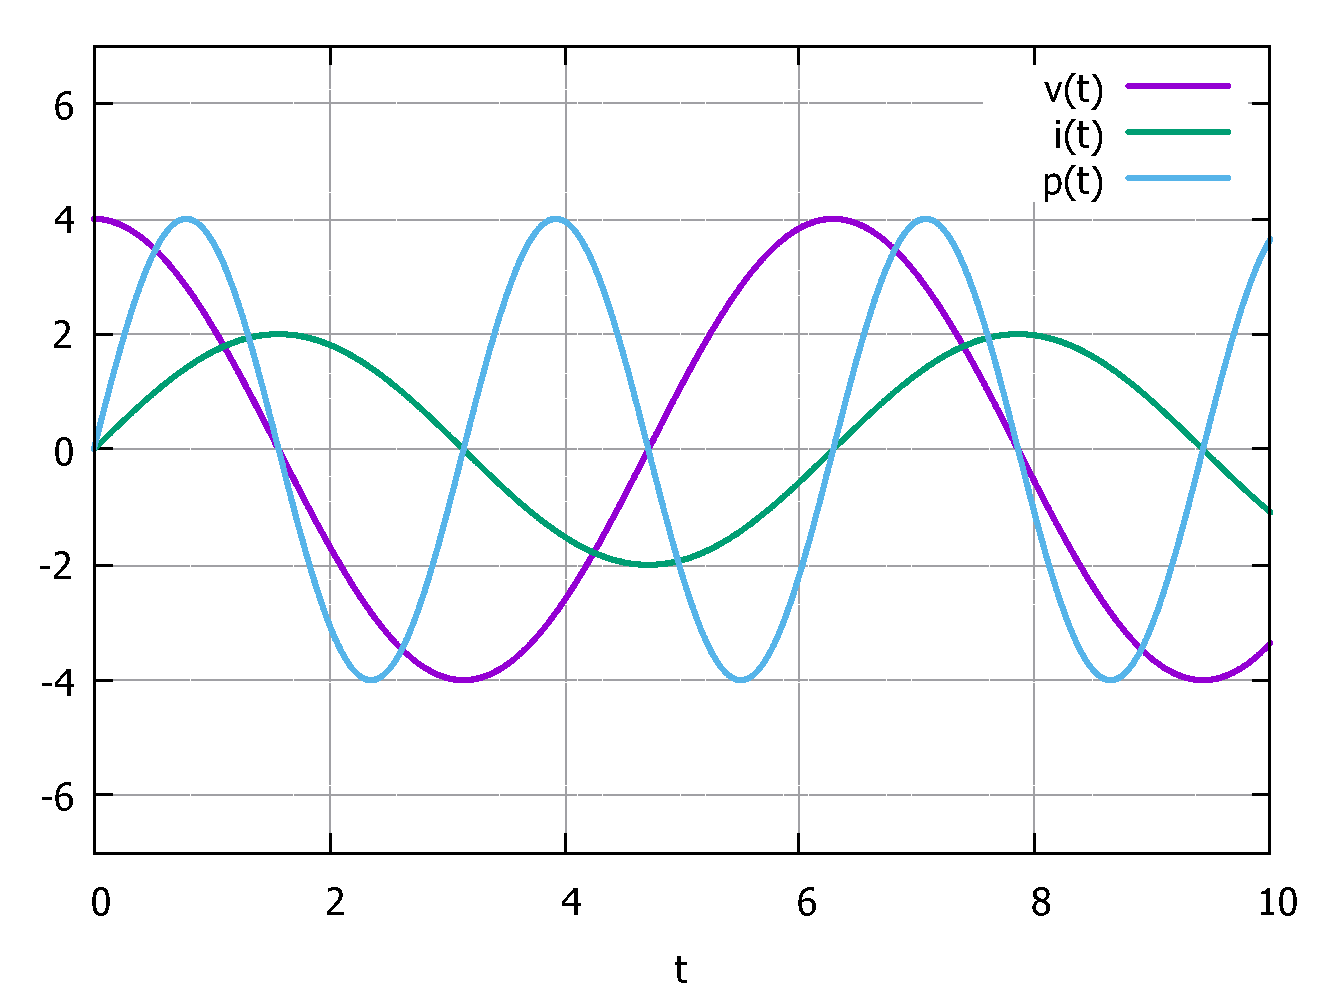
\includegraphics[scale=0.4]{potenciainduccion.pdf}
\caption{Potencia a través de una bobina pura}
\end{figure}



por lo que el valor medio $P$ de la potencia que atraviesa una resistencia pura será de $\frac{1}{2} V_m I_m$. Para un circuito cualquiera el desfase será un ángulo $\theta$ cualquiera, de tal modo que la potencia vendrá dada por:

\begin{equation}
p(t) = V_m I_m \sin (wt) \sin (wt + \theta)
\end{equation}
y aplicando el producto de senos:

\begin{equation}
p = \dfrac{1}{2} V_m I_m [\cos (\theta) - cos(2wt+\theta)]
\end{equation}

El valor medio de la potencia será entonces:

\begin{equation}
P = \dfrac{1}{2} V_m I_m \cos (\theta) = V I \cos (\theta)
\end{equation}
donde llamamos $V = V_m/\sqrt{2}, I = I_m / \sqrt{2}$ a los \textbf{valores eficaces}. Llamamos al término $\cos ( \theta )$ el \textbf{factor de potencia}. El ángulo $\theta$ estará siempre comprendido entre $-\pi/2$ y $\pi/2$ de tal forma que $P$ siempre es positivo. Indicaremos el símbolo de $\theta$ de la siguiente manera: si es negativo diremos que estamos en un \textit{circuito inductivo} y si es positivo \textit{circuito capacitivo}. 


\subsubsection{Potencia aparente y reactiva}

Llamamos \textbf{potencia aparente} $S$ al producto de los valores eficaces de tal forma que:

\begin{equation}
S = VI
\end{equation}
y llamamos \textbf{potencia reactiva} $Q$ al producto de los valores eficaces por el seno de $\theta$:

\begin{equation}
Q = VI \sin (\theta)
\end{equation}

\subsubsection{Potencia compleja}

Esto que acabamos de definir se puede ver muy bien si creamos una potencia compleja, cuyo módulo será igual a la potencia aparente. Esta potencia compleja la denotaremos por $S$, de tal forma que:

\begin{equation}
S = V I^* = Ve^{j \alpha} I e^{-j(\alpha + \theta)} = VI e^{j \theta} = VI \cos (\theta) - j VI \sin (\theta) = P - j Q
\end{equation}
La parte real de la potencia compleja será la potencia activa, la parte compleja será la potencia reactiva y el módulo la potencia aparente. Esto se puede representar en los lados de un triángulo en lo que llamamos el \textit{triángulo del potencial}.


\subsection{Resonancia en serie y paralelo}

Como hemos visto la impedancia de un circuito RLC se puede expresar como:

\begin{equation}
Z = R + j (wL-1/wC) = R + j X
\end{equation}

\begin{figure}[h!] \centering
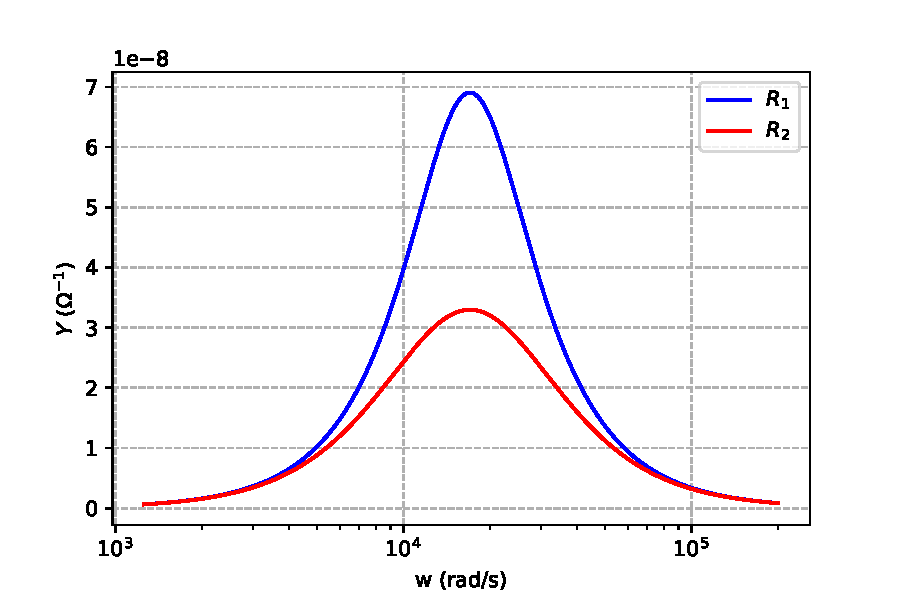
\includegraphics[scale=0.8]{amictancia.pdf}
\end{figure}

\begin{figure}[h!] \centering
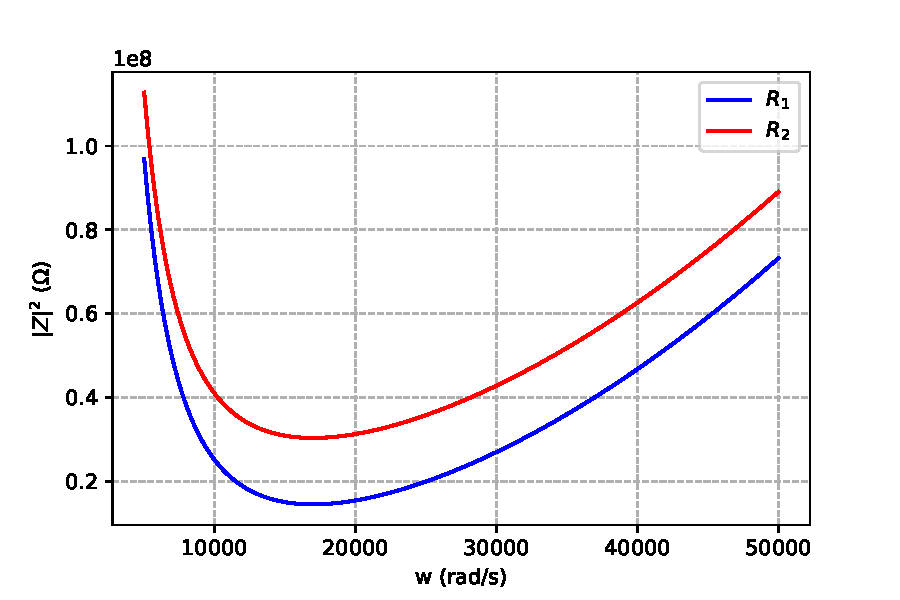
\includegraphics[scale=0.8]{impedancia.pdf}
\end{figure}

\begin{figure}[h!] \centering
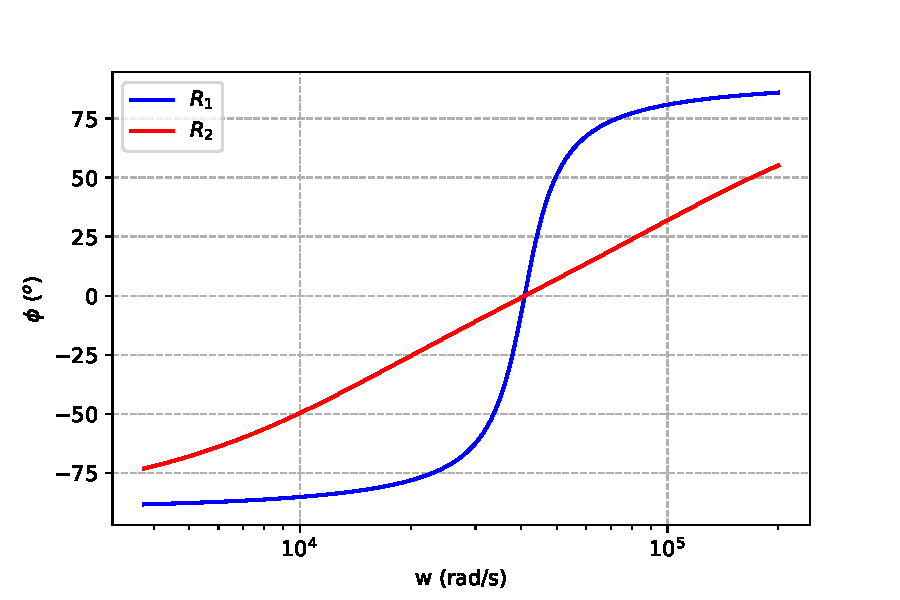
\includegraphics[scale=0.8]{desfase.pdf}
\end{figure}


donde llamamos a $X$ la \textbf{reactancia}. Como ya hemos mencionado, existe una frecuencia para la cual la reactancia se anula, que viene dada por $w_0 = 1/\sqrt{LC}$. Cuando estamos en esta frecuencia se dice que nuestro circuito ha entrado en \textit{resonancia}. Dado que $2 \pi f = w$ definimos como \textbf{frecuencia de resonancia} a:

\begin{equation}
f = \dfrac{1}{2 \pi \sqrt{LC}}
\end{equation}




Además de definir la frecuencia de resonancia existen otros parámetros tales como el ancho de banda o el factor de calidad de un circuito que tienen valores concretos en un circuito RLC. El factor de calidad de un circuito se define como:

\begin{equation}
Q  = 2 \pi \ \dfrac{\mathrm{energia \ maxima \ almacenada}}{\mathrm{energia \ disipada \ por \ periodo}}
\end{equation}

y se puede definir, en un circuito RLC como:

\begin{equation}
Q = \dfrac{w_0 L}{R} = \dfrac{1}{w_0 RC}
\end{equation}

Es un factor adimensional. ancho de banda de un circuito RLC es la diferencia entre las frecuencias $w_1$ y $w_2$ para las cuales la intensidad de la señal cae la raíz cuadrada de la máxima señal (que es cuando está en resonancia). Entonces:

\begin{equation}
B = w_2 - w_1
\end{equation}

que sí tiene dimensiones (de frecuencia). Se pueden demostrar las siguientes relaciones (se puede cambiar $f$ por $w$):

\begin{equation}
Q = \dfrac{f_0}{f_2  - f_1}; \tquad f_0 = \sqrt{f_1 f_2}
\end{equation} 


\subsection{Teorema de Superposición}

El \textbf{teorema de superposición} establece que la respuesta en cualquier elemento de un circuito lineal bilateral que contenga dos o más fuente es la suma de las respuestas obtenidas para cada una de las fuentes actuando separadamente y con todas las demás fuentes igual a cero. \\

Este principio de superposición está implícito en los métodos de análisis por las corrientes de mallas y las tensiones de los nudos. Es extremadamente útil cuando los generadores de corriente y generadores de intensidad aplican señales de frecuencias diferentes. La manera de obviar los generador es muy obvia:

\begin{itemize}
\item \textit{Generador de tensión:} se tratará de substituir dicho generador por una caída de tensión 0. Esto se consigue haciendo un cortocircuito al generador, es decir, sustituyendo dicho generador por un cable.
\item \textit{Generador de corriente:} se tratará de substituir dicho generador por una corriente cero en el brazo. Esto se consigue poniendo en circuito abierto a dicho generador.
\end{itemize}

La potencia no se puede hallar por superposición ya que la relación entre potencia y corriente con la tensión es cuadrática.

\subsubsection{Teorema de transferencia máxima}

Supongamos una red lineal, tal que salgan dos terminales hacia una resistencia $Z_L$. Por el teorema de Thevenin podemos substituir toda la red lineal por una tensión Thevenin $V_h$ y una impedancia equivalente $Z_{th}$. El teorema de transferencia máxima nos da una medida de cuál tiene que ser el valor de la impedancia para la cual somos capaces de proporcionar la mayor potencia activa posible al elemento $Z_L$.  \\

Para esto está claro que:

\begin{equation}
V_{th} + I(Z_{th}+R_L + j X_L) = 0 \Longrightarrow I = \dfrac{V}{(R_{th}+R_L)+j(X_{th}+X_L)}
\end{equation}

La potencia activa que se consume viene dada por:

\begin{equation}
P_L = |I|^2 R_L = \dfrac{|V_{th}|^2 R_L}{(R_{th}+R_L)^2+(X_{th}+X_L)^2}
\end{equation}

Para que sea máxima la máxima dado que la parte resistiva no puede ser negativa se debe verificar que:

\begin{equation}
X_L = -X_{th} 
\end{equation}

Además si se verifica esta condición tenemos que:

\begin{equation}
R_L = R_{th}
\end{equation}

Por lo tanto se debe verificar que para que haya una transferencia máxima de potencia se debe verificar que $Z_L = Z_{th}^*$. Así para calcular que impedancia que hay que colocar en una parte del circuito para obtener la mayor potencia activa posible, tenemos que calcular la impedancia Thevenin y hacer su complejo conjugado

\newpage

\section{Lineas de trasmisión}

Una línea de trasmisión no es otra cosa que un circuito para el cual las longitudes son tan grandes que no podemos hacer una aproximación estacionaria. En general las líneas de tramisión son tan grades o más como la longitud de onda de la señal.  \\

En general una línea de trasmisión es un cable coaxial, ya que para una propagación TEM (modo trasversal electromagnético) la línea de trasmisión debe de tener dos conductores. Un ejemplo común de línea de trasmisión es un cable coaxial, ya que los campos electromagnéticos estarán completamente encerrados, y serán perpendiculares. \\


\begin{figure}[h!] \centering
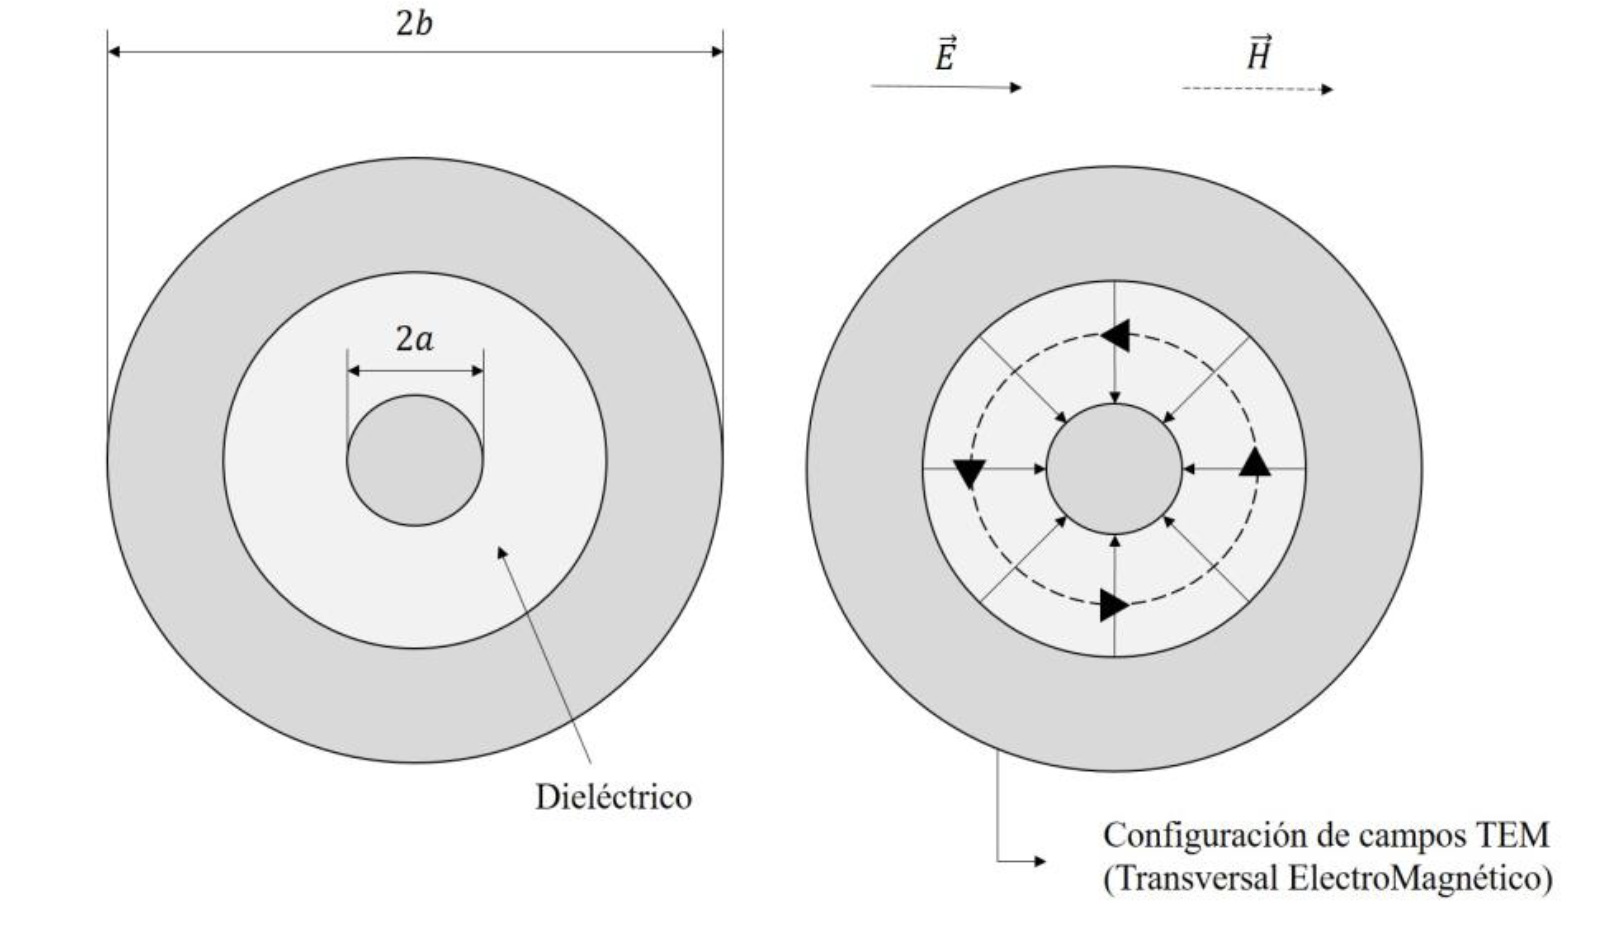
\includegraphics[scale=0.5]{lineatrasmision1.png}
\end{figure}


En este caso el campo eléctrico tendrá dirección radial y el campo magnético dirección angular. Además por simetría los campos serán independientes del ángulo $\phi$. El operador Laplaciano trasversal en cilíndricas viene dado por:

$$ \nabla^2 = \dfrac{1}{r} \dfrac{\D}{\D r} \parentesis{r \dfrac{\D }{\D r}} $$
 
Por lo que nuestro problema será resolver la ecuación del potencial $\Phi$ tal que se debe verificar $\nabla^2 \Phi = 0$. Como condiciones de frontera tenemos que: $\Phi (a) = 0, \Phi (b) = V_0$, por lo que el potencial vendrá dado por:

\begin{equation}
\Phi (r) = V_0 \dfrac{\log (r/a)}{\log (b/a)}
\end{equation} 

una vez hemos resulto la ecuación diferencial y aplicado las condiciones de contorno. Como nuestro potencial viene dado por esa función y se verificará que $\vec{E} = - \nabla \Phi e^{j(wt-kz)}$, tenemos que:

\begin{equation}
\vec{E} = - \dfrac{V_0}{\log(b/a)} \dfrac{\hat{r}}{r} e^{k(wt-kz)}
\end{equation}

Suponiendo que por el conductor interior circule una corriente a $I_0$ tenemos que:

\begin{equation}
\vec{H} = \dfrac{I_0}{2 \pi r} \hat{\phi}  e^{j(wt-kz)} 
\end{equation}

que podemos relacionar con $\vec{E}$ tal que:

\begin{equation}
\vec{H} = \dfrac{-V_0 / Z_{tem}}{\log ( b/a)} \dfrac{\hat{\phi}}{r} e^{j(wt-kz)}
\end{equation}

tal que $Z_{tem} = \eta_v / \sqrt{\epsilon_r}, \ \eta_v = \sqrt{\mu_0 / \epsilon_0}$



\subsection{Modelo circuital de parámetros distribuidos}

Ahora vamos a tratar de relacionar los parámetros de un circuito con las líneas de trasmisión, ya que como hemos dicho, una línea de trasmisión no es mas que un circuito muy grande. Considerando una longitud diferencial $\Delta z$ tal que:

\begin{figure}[h!] \centering
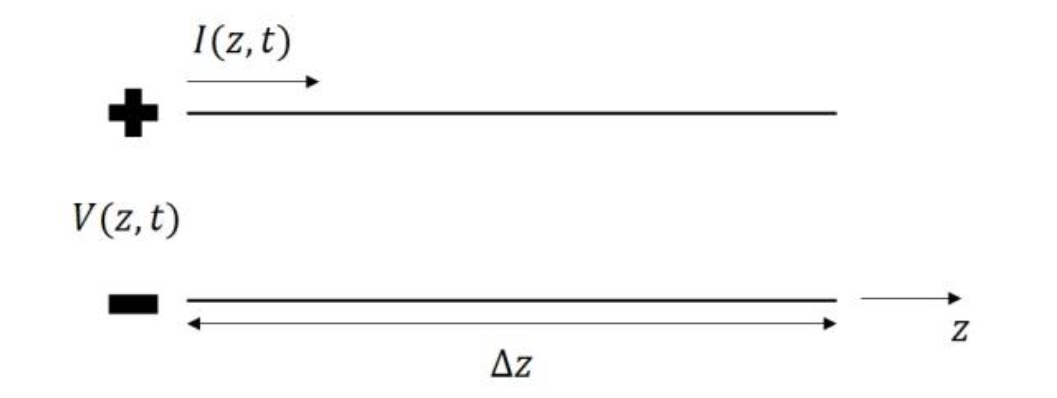
\includegraphics[scale=0.5]{lineatrasmision2.png}
\end{figure}


Podemos modelizar la línea de trasmisión como un circuito tal que:


\begin{figure}[h!] \centering
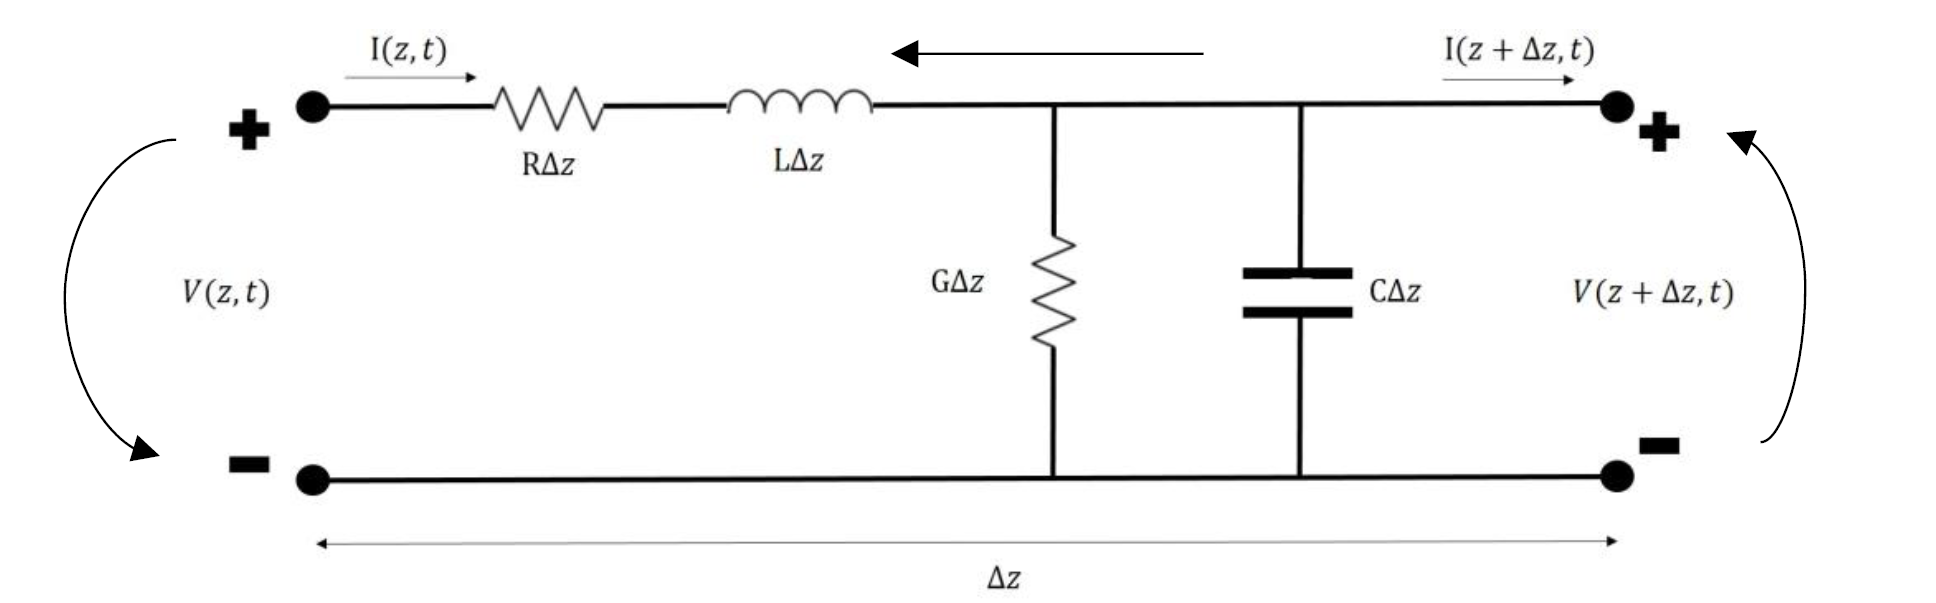
\includegraphics[scale=0.5]{lineatrasmision.png}
\end{figure}



Donde tenemos los siguientes significados:

\begin{itemize}
\item $R$: es la resistencia por unidad de longitud. Representa la resistencia debida a al conductividad finita de los conductores.

\item $L$: es la inductancia por unidad de longitud. Representa la inductancia mutua entre ambos conductores. 

\item $G$: es la conductancia por unidad de longitud. Representa las pérdidas eléctricas dieléctricas en el material entre conductores.

\item $C$: es la capacidad por unidad de longitud. Representa la capacidad entre conductores separados por el dieléctrico.
\end{itemize}
 
Ahora resolvemos la ecuación del circuito por mallas y nudos:

\begin{equation}
-(R+jwL)I(z,t)\Delta z = V(z+\Delta z,t) - V(z,t)  \label{Ec:8.1-001}
\end{equation}

\begin{equation}
I(z,t)= I(z+\Delta z,t) + V(z,t)(G+jwC) \Delta z \label{Ec:8.1-002}
\end{equation}

Ahora si $\Delta z \rightarrow 0$ las ecuaciones se transforman en:

\begin{equation}
\parciales{V(z,t)}{z} = - (R+jwL)I(z,t)
\end{equation}
\begin{equation}
\parciales{I(z,t)}{z} = - (G+jwC)V(z,t)
\end{equation}
 
donde hemos aplicado la definición de derivada parcial. Si volvemos a derivar respecto a $z$ (en cada lado), podemos ver que tanto $V$ como $I$ verifican la misma ecuación diferencial de mismo orden:

\begin{equation}
\parciales{^2 V(z,t)}{z^2} = (R+jwL)(G+jwC)V(z,t)
\end{equation}
 
por lo que nuestro potencial vendrá dado por:

\begin{equation}
V(z,t) = A \cdot e^{jwt-\gamma z} + B \cdot e^{jwt + \gamma z}
\end{equation}

donde $A$ y $B$ son constantes que dependen de las condiciones iniciales del problema, y $\gamma$ es un número complejo tal que:

\begin{equation}
\gamma = \alpha + j \beta = \sqrt{(R+jwL)(G+jwC)}
\end{equation}

Dado que la intensidad está acoplada al potencial según las ecuaciones  \ref{Ec:8.1-001} y \ref{Ec:8.1-002} tenemos que está vendrá dada por:

\begin{equation}
I(z,t) = \dfrac{A}{Z_0} e^{jwt-\gamma z} - \dfrac{B}{Z_0} e^{jwt+\gamma z}
\end{equation}
 
donde $Z_0$ es la \textbf{impedancia característica} del medio tal que:

\begin{equation}
Z_0 = \sqrt{\dfrac{R+jwL}{G+jwC}}
\end{equation}
 
Si nos paramos a pensar un poco que $\gamma$ sea un número complejo que dependa de los parámetros de la línea de trasmisión tiene sentido, ya que una señal no se trasmitirá igual por un conductor de cobre que de acero que de oro. Como cada uno de estos tiene una resistencia por unidad longitud diferente, evidentemente la señal no se puede propagar de la misma forma. Lo mismo si tenemos los conductores muy juntos o muy separados (afectando a la capacidad) o un dieléctrico u otro (afecta también a la capacidad). Lo mismo ocurre con $Z_0$: en función de los parámetros de la línea de trasmisión la relación intensidad-voltaje cambiará. \\

Siempre que sea posible calcular $R$,$L$,$C$,$G$; se podrá deducir $\alpha,\beta,Z_0$, y todo lo que conlleva ello. Por ejemplo un medio sin pérdidas (ideal) tal que $R=G=0$ implica que:

\begin{equation}
\gamma = \sqrt{-w^LC}; \ \ \ \ \ \ v_p = \dfrac{w}{k} = \dfrac{w}{\beta} = \dfrac{1}{\sqrt{LC}}
\end{equation}

\subsection{Capacidad e inductancia cable coaxial}

Si nuestra línea de trasmisión es un cable coaxial podemos calcular fácilmente la inductancia y la capacidad por longitud de cable. Estas vienen dadas por:

\begin{equation}
C = \dfrac{2 \pi \epsilon}{\log (b/a)} \tquad L = \dfrac{\mu_0}{2 \pi} \log (b/a)
\end{equation}

Por lo que la velocidad de propagación de la onda será:

\begin{equation}
v_p = \dfrac{1}{\sqrt{\mu_0 \epsilon}} = \dfrac{c}{\sqrt{\epsilon_r}}
\end{equation}

y la impedancia característica:

\begin{equation}
Z_0 = \sqrt{\frac{L}{C}} = \dfrac{\log(b/a)}{2 \pi } \sqrt{\frac{\mu_0}{\epsilon}}
\end{equation}

Lo que vamos a definir a continuación es importante: definimos como \textbf{coeficiente de reflexión} $\rho$ a

\begin{equation}
\rho = \dfrac{B \cdot e^{\gamma l}}{A \cdot e^{-\gamma l}} = |\rho| \cdot e^{j \phi} = \dfrac{Z_L - Z_0}{Z_L + Z_0}
\end{equation}
 
entonces si $Z_0 \neq Z_L$ siendo $Z_L$ la impedancia al final del circuito (véase la figura) aparecerán ondas reflejadas y ondas estacionarias
 

\begin{figure}[h!] \centering
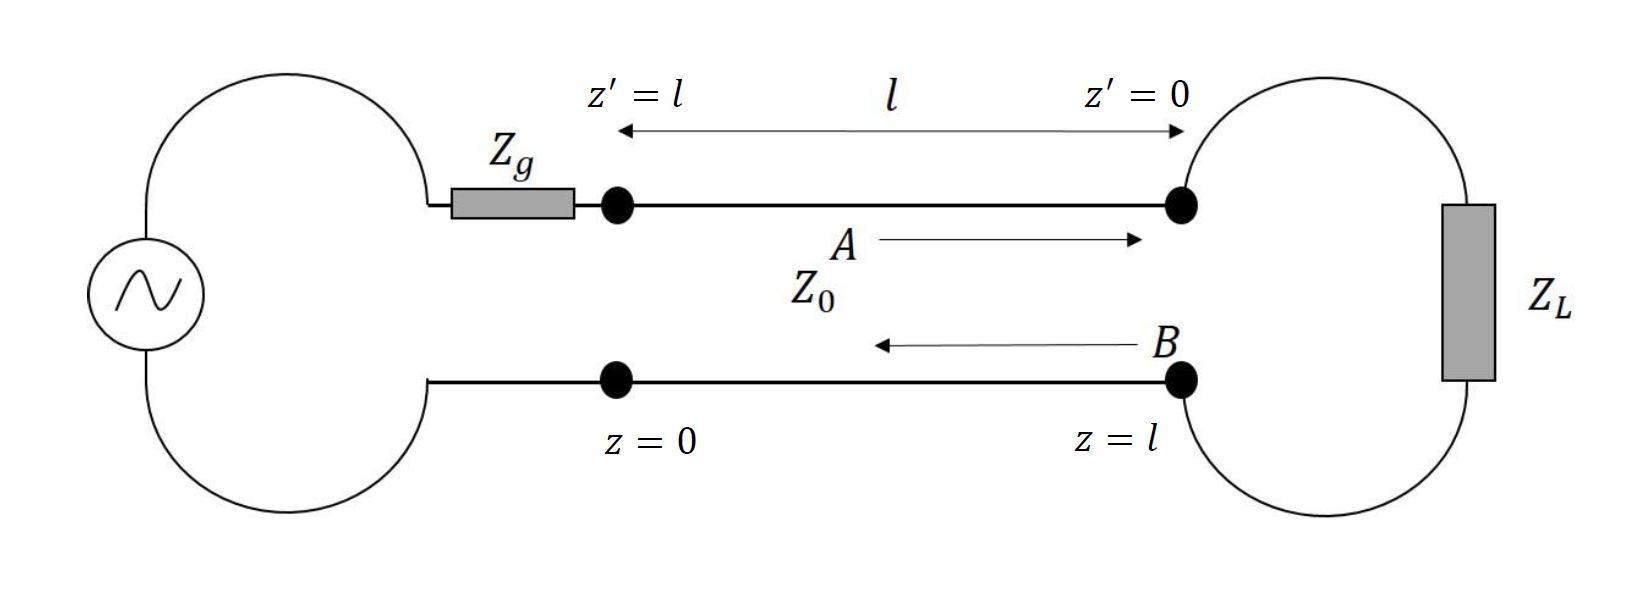
\includegraphics[scale=0.5]{lineatrasmision3.png} \label{Fig:8.2-004}
\caption{Línea de tramisión}
\end{figure}

 
\subsection{Distribución de corriente en un dipolo}

En la teoría de líneas de trasmisión es de utilidad calcular la distribución de corriente en un dipolo alimentado centralmente, por diversas razones que comentaremos mas adelante. Sin embargo es posible que no se sepa que es un dipolo en el estudio de parámetros distribuidos. \\

Un \textbf{dipolo} es un tipo de antena que consta de dos elementos conductores separados y alimentados centralmente. Estos elementos pueden ser alambres, varillas o cualquier otro tipo de conductor. El dipolo se caracteriza por tener una longitud que es aproximadamente la mitad de la longitud de onda de la señal que se va a transmitir o recibir. Se utiliza para la transmisión y recepción de señales de radiofrecuencia. Es quizás la antena mas simple pero también mas usada en líneas de trasmisión. \\

Gráficamente se puede ver como un par de conductores tubulares de diámetro $d$ tal que $d\ll \lambda,2l$:


\begin{figure}[h!] \centering
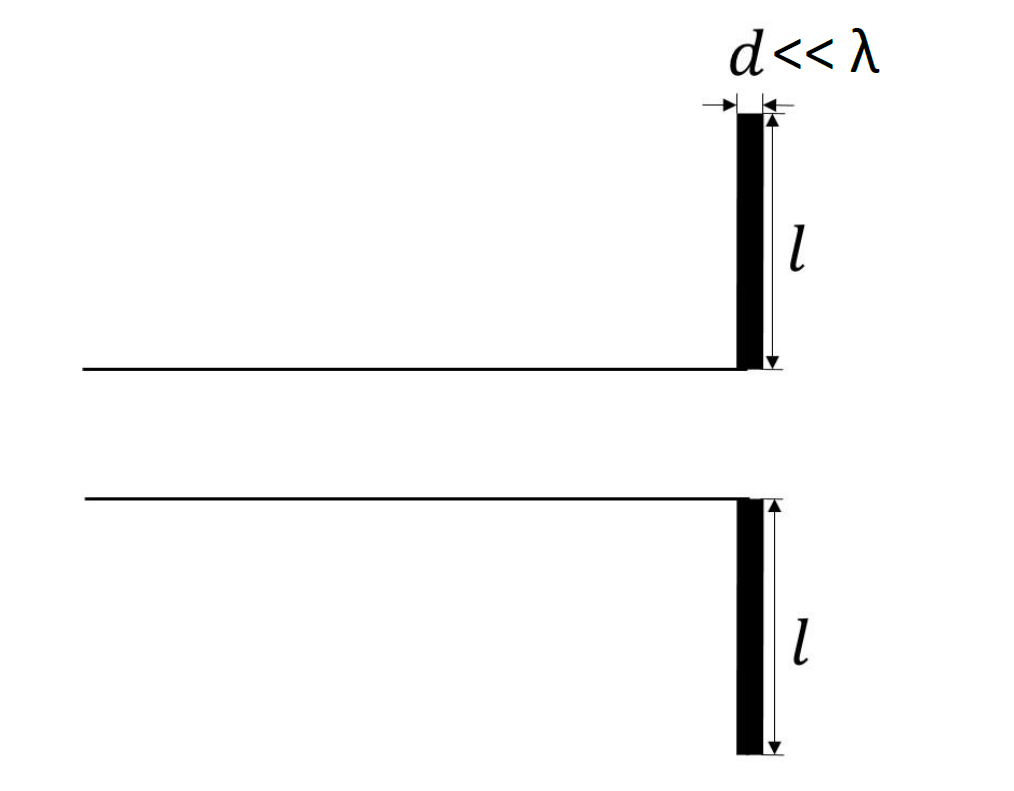
\includegraphics[scale=0.5]{lineatrasmision4.png}
\end{figure}

A través del hueco se le aplica un voltaje apareciendo una distribución de corriente sobre el par de conductores. Esta misma corriente es la que va a producir un campo radiante. \\

Si consideramos la figura \ref{Fig:8.2-004} tal que está abierto ($Z_L = \infty$), teneos que $|\rho| = 1$, y por lo tanto $A=B$. Si la distancia entre conductores permanece constante la terminación en abierto produce una distribución de corriente de onda estacionaria en oposición en los dos conductores y prácticamente no produce radiación. \\

Como la corriente al final de la línea de trasmisión no puede trasmitirse (está en abierto el circuito) claramente la señal se reflejará para que justo en el punto $x=l$ (final de la línea) la intensidad sea siempre cero. Si consideramos que el origen de $x$ está a una distancia de $l$ del final tenemos que:

\begin{equation}
I (x,t) = \dfrac{A}{Z_0 } e^{j(wt - k(l-x))} - \dfrac{A}{Z_0 } e^{j(wt - k(l-x))} = - \dfrac{2 A j}{Z_0} e^{jwt} \cdot \sin (k(l-x))
\end{equation}

Ahora bien si vamos abriendo este dipolo tanto las inductancias como las capacidades por unidad de longitud van a ir cambiando a lo largo del segmento inclinado. Si llegamos a una apertura de 180 grados el dipolo generará una radiación electromagnética (emitirá ondas electromagnéticas al exterior). Sin embargo suponemos que el número de onda si es constante, lo que implica que solo variará el máximo de corriente estacionaria, y no su comportamiento sinusoidal.


\subsection{Coeficiente de reflexión}

Como se ha definido, el coeficiente de reflexión viene dado por:

$$ \rho = \dfrac{B \cdot e^{\gamma l}}{A \cdot e^{-\gamma l}} = |\rho| \cdot e^{j \phi} $$

Para $x=l$ se verificará que $B e^{\gamma l} = \rho A e^{-\gamma l}$. Por esa razón:

\begin{equation}
V(l) = A e^{-\gamma l} (1+ \rho)
\end{equation}

\begin{equation}
I(l) = \frac{A}{Z_0} e^{-\gamma l} (1-\rho)
\end{equation}

Definimos como impedancia en los extremos como el cociente entre el voltaje e intensidad para $x=l$ tal que $Z_L = V_l / I_l = Z_0 \frac{1+\rho}{1-\rho}$. Entonces se puede deducir por esta ecuación que:

\begin{equation}
\rho = \frac{Z_L - Z_0}{Z_L+Z_0}
\end{equation}

\subsection{Relación de tensión en la onda estacionaria}

Cuando una línea de trasmisión termina en una impedancia arbitraria aparecen una onda incidente y reflejada, con diferentes amplitudes. Si $A$ y $B$ son sus respectivas amplitudes, el máximo ($V_{max} = A+B$) se produce cuando en algún punto de la línea las dos amplitudes están en fase, y el mínimo ($V_{min} = A-B$) donde se presenta un desfase. Definimos como \textbf{razón de onda estacionaria} a la diferencia entre el voltaje máximo y mínimo:

\begin{equation}
S = \dfrac{|V_{max}|}{|V_{min}|} = \dfrac{A+B}{A_B} = \dfrac{1+B/A}{1-B/A} = \dfrac{1+|\rho |}{1-|\rho|}
\end{equation}

\subsection{Expresiones de campo lejano para antenas}

Cuando las fuentes que generan una señal (campos) están muy lejos de donde los medimos, podemos simplificar mucho las expresiones que relacionan campo-fuente. Como ya hemos dicho queremos calcular $\vec{E}$ y $\vec{B}$ en el punto $\vec{r} = (x,y,z)$ situados lejos de las fuentes (de ahora en adelante coordenadas primadas) $\vec{r}'=(x',y',z')$ tal que si $R$ es la distancia de $\vec{r}$ a $\vec{r}'$, $R \gg |r'|$.\\


Entonces dado que las fuentes están suficientemente lejos,  si estás oscilan armónicamente a una frecuencia angular $w$ contenidas en un volumen finito $V$, podemos aproximar las ecuaciones de Maxwell:

\begin{equation}
\rota \vec{E} = -  j w \vec{B}; \tquad \rota \vec{B}  = \dfrac{j w}{c^2} \vec{E}; \tquad \dive \vec{E} = 0; \tquad \dive \vec{B} = 0
\end{equation}

Como sabemos para fuentes estacionarias podemos relacionar:

\begin{equation}
\vec{B} = \rota \vec{A}
\end{equation}

tal que el potencial vectorial viene dado por:

\begin{equation}
\vec{A}(\vec{r},t) = \dfrac{\mu_0}{4 \pi} \int_V \dfrac{\vec{J} (\vec{r'}) e^{j(wt-kR)}}{R} \D V
\end{equation}

Si expresamos $R$ como:

$$ \begin{array}{lll} 
R & = & |\vec{r}-\vec{r'}| = [(r \sin \theta \cos \phi - x')^2 + (r \sin \theta \sin \phi - y')^2 + (r\cos\theta-z')^2]^{1/2}\\
 & = & r - (x' \sin \theta \cos \phi + y' \sin \theta \sin \phi + z' \cos \phi) + \eta(r^{-1}) + \cdots
\end{array}  $$

Donde hemos hecho una expansión por taylor cendrada en $r$. Despreciando cualquier término mayor que $r^{-1}$, tenemos que $\vec{A}$ se puede aproximar a:

\begin{equation}
\vec{A} (x,y,z,t) = \dfrac{\mu_0 \cdot e^{j(wt-kr)}}{4 \pi \cdot  r} \int_V \vec{J} (\vec{r}') e^{jkL} \D V
\end{equation} 

donde $L = (x' \sin \theta \cos \phi + y' \sin \theta \sin \phi + z' \cos \phi)$, que puede interpretarse como el \textit{producto escalar} de \textit{el vector posición desde el origen al punto fuente} ($x',y',z'$). \\
 
Entonces $\vec{A}$ viene dado por el producto de dos factores: una onda esférica (todo lo que va con la exponencial fuera de la integral) por una función ponderada $\vec{a}$ que depende de $\phi$ y de $\theta$  (la integral) tal que:

\begin{equation}
\vec{a} (\theta,\phi) = \int_V \vec{J} (x',y',z') e^{ikL} \D x' \D y' \D z'
\end{equation}

Tenemos que:

\begin{equation}
\vec{A} = \dfrac{\mu_0 \cdot e^{j(wt-kr)}}{4 \pi \cdot  r} \ \vec{a} (\theta,\phi)
\end{equation}

que por lo tanto tenemos que para los campos:

\begin{equation}
\vec{E} = (c^2/j w) \rota \rota \vec{A} = jw \ \hat{r} \times (\hat{r} \times \vec{A}) = - j w \vec{A}_T
\end{equation}
\begin{equation}
\vec{H} = (\mu^{-1}) \rota  \vec{A} = - \parentesis{\dfrac{jw}{\eta}} \hat{r} \times \vec{A} = \parentesis{\dfrac{1}{\eta}} \hat{r} \times \vec{E}
\end{equation}

donde $\eta$ es la impedancia característica del medio, y $\vec{A}_T = A_\theta \hat{\theta} + A_\phi \hat{\phi}$ (ya que obviamente lo que vaya con $\hat{r}$   desaparecerá por el producto vectorial). Si ahora  calculamos el vector de Poyting:

\begin{equation}
\vec{S} = \dfrac{1}{2} \mathrm{Re} (\vec{E} \times \vec{H}^*) \hat{r} = \hat{r} \ccorchetes{\frac{k^2 \eta}{(4 \pi r^2)}} \cdot \ccorchetes{\dfrac{1}{2} a_{\theta} a_\theta^* + \dfrac{1}{2} a_\phi a_\phi^*} 
\end{equation}

Entones el vector $\vec{a}$ está relacionado con la densidad de energía y flujo. A la parte del campo $E$ que va con $\phi$ se le llama patrón polarizado horizontalmente, y el que va con $\theta$ patrón polarizado verticalmente. Los vectores vendrán dados por:

\begin{equation}
a_\theta (\theta, \phi) = \int_V [\cos \theta \cos \phi J_x + \cos \theta \sin \phi J_y - \sin \theta J_z] e^{jkL} \D x' \D y' \D z'
\end{equation}
\begin{equation}
a_\phi (\theta, \phi) = \int_V [\sin \phi J_x +  \cos \phi J_y ]e^{jkL} \D x' \D y' \D z'
\end{equation}


\subsection{Propiedades radiantes de un dipolo}

Ahora podemos resolver las ecuaciones del campo para un dipolo, ya que conocemos su distribución de corrientes y por lo tanto podremos integrar y hallar $\vec{a}$. Para recordarlo tenemos que la intensidad de una antena:

\begin{equation}
I(x,t) = I_m \sin [k(l-x)] e^{jwt}
\end{equation}
tal que entones $\vec{J} || \hat{z}$ de lo que se deduce que: 

\begin{equation}
a_\theta = - I_m \sin \theta \int_{-L}^L \sin [k (l - |z'|)] e^{jkz \cos \theta} \D z'; \tquad a_\phi=0
 \end{equation}
e integrando:

\begin{equation}
a_\theta(\theta) = - \dfrac{2 I_m}{k \sin \theta} [ \cos (kl \cos \theta) - \cos (kl)]
\end{equation}



Si la longitud de el dipolo es la mitad de la longitud de la onda tal que $2l = \lambda / 2  = \pi/k$, por lo que:

\begin{equation}
a_{\theta} (\theta) = - \dfrac{2 I_m}{k} \dfrac{\cos (\frac{\pi}{2} \cos \theta)}{\sin \theta}
\end{equation}
 
Para un dipolo de estas características el patrón de ondas viene dado por:

\begin{equation}
E_\theta (\theta) = j 60 I_m \dfrac{e^{j(wt-kr)}}{r} \ccorchetes{\dfrac{\cos \ccorchetes{\parentesis{\frac{\pi}{2}} \cos \theta}}{\sin \theta}}
\end{equation}

\begin{equation}
H_\phi (\theta) = j  \dfrac{I_m}{2 \pi} \dfrac{e^{j(wt-kr)}}{r} \ccorchetes{\dfrac{\cos \ccorchetes{\parentesis{\frac{\pi}{2}} \cos \theta}}{\sin \theta}}
\end{equation}

El patrón de potencia:


\begin{equation}
P_{r,\theta} (\theta,\phi) = \dfrac{2 \eta I_m^2}{(4 \pi r)^2} \ccorchetes{\dfrac{cos^2 \ccorchetes{\parentesis{\pi/2} \cos \theta}}{\sin^2 \theta}}
\end{equation}
 
Si integramos en todo el espacio llegamos a la potencia total irradiada por la antena. Definimos como \textit{directividad máxima} de un dipolo $\lambda/2$ a:

\begin{equation}
D = 4 \pi r^2 \dfrac{P_{r,\theta} (\pi/2)}{P_{rad}}
\end{equation} 
 
 
\end{document}



